\SourcePage{25}
\section*{1.1. 三角范畴}
\addcontentsline{toc}{section}{1.1. 三角范畴}
关于\term{triangulated-category}{三角范畴}的定义与基本性质，参见 J. L. Verdier [10]。本节旨在说明 Verdier 的公理，特别是\term{octahedral-axiom}{八面体公理}，并给出一些补充。

\par\medskip\noindent\textbf{1.1.1.} 一个\term{triangulated-category}{三角范畴}是一个\term{additive-category}{加性范畴} $\mathcal D$，配备\term{shift-functor}{平移函子} $X\mapsto X[1]$ 和一族“三角” $X\to Y\to Z\to X[1]$，称为\term{distinguished-triangle}{区别三角}。要求\term{shift-functor}{平移函子}是范畴的自\term{equivalence}{等价}，并要求\term{distinguished-triangle}{区别三角}族满足 [10] 第4页的公理 TR 1 至 TR 4。

\term{shift-functor}{平移函子}的第 $n$ 次迭代记为 $X\mapsto X[n]$（$n\in\Z$）。在图中，次数为 $n$ 的箭头标注 $(n)$。\term{distinguished-triangle}{区别三角}常写成线性形式
\[
 X\longrightarrow Y\longrightarrow Z\xrightarrow{(1)}
 \qquad\text{（或简记为 $(X,Y,Z)$）},
\]
它代表
\[
\begin{tikzcd}[ampersand replacement=\&,column sep=small,row sep=small]
 \& Z\arrow[dl,"{(1)}"']\&\\
 X\arrow[rr]\&\&Y\arrow[ul]
\end{tikzcd}
\]
不致混淆时，省略一次箭头上的 $(1)$。约定 $\Hom^n(X,Y):=\Hom(X,Y[n])$。

$\mathcal D$ 的\term{duality}{对偶}范畴 $\mathcal D^{\mathrm{opp}}$ 配备由 $X\mapsto X[1]$ 的逆函子诱导的\term{shift-functor}{平移函子}。因此，$\mathcal D$ 中一个次数为 $n$ 的箭头 $X\to Y$，在 $\mathcal D^{\mathrm{opp}}$ 中给出从 $Y$ 到 $X$ 的同次数箭头。$\mathcal D^{\mathrm{opp}}$ 的\term{distinguished-triangle}{区别三角}定义为 $(Z,Y,X)$，其中 $(X,Y,Z)$ 是 $\mathcal D$ 中的\term{distinguished-triangle}{区别三角}。如此，$\mathcal D^{\mathrm{opp}}$ 成为\term{triangulated-category}{三角范畴}，这使我们可以使用\term{duality}{对偶}论证。

在\term{triangulated-category}{三角范畴}中，每个态射 $f:X\to Y$ 都是某个\term{distinguished-triangle}{区别三角} $(X,Y,Z)$ 的底边；这样的三角在同构意义下唯一，但同构一般并不唯一（关于唯一性的一个情形，见1.1.10）。称第三个顶点 $Z$ 为 $f$ 的\term{cone}{锥}（更准确地说，是它的一个\term{cone}{锥}）。\term{distinguished-triangle}{区别三角} $(X,Y,Z)$ 对任意 $T$ 都给出\term{exact-sequence}{正合列}
\[
 \begin{gathered}
 \Hom(T,X)\to\Hom(T,Y)\to\Hom(T,Z),\\[3pt]
 \Hom(Z,T)\to\Hom(Y,T)\to\Hom(X,T).
 \end{gathered}
\]
由于\term{distinguished-triangle}{区别三角}可以旋转，即公理 TR 2 断言
\[
 X\xrightarrow{u}Y\xrightarrow{v}Z\xrightarrow{d}X[1]
 \quad\Longleftrightarrow\quad
 Y\xrightarrow{v}Z\xrightarrow{d}X[1]\xrightarrow{-u[1]}Y[1]
\]
两边同时为\term{distinguished-triangle}{区别三角}，这些\term{exact-sequence}{正合列}
\SourcePage{26}
可以延长为长\term{exact-sequence}{正合列}。

\term{triangulated-category}{三角范畴}的公理来自下面1.1.2至1.1.5中的例子。

\par\medskip\noindent\textbf{1.1.2.} 设 $A$ 是\term{additive-category}{加性范畴}。定义范畴 $KA$ 如下：对象是 $A$ 中对象构成的\term{complex}{复形}，$\Hom_{KA}(K,L)$ 是从 $K$ 到 $L$ 的\term{complex}{复形}态射的\term{homotopy}{同伦}类集合。$K$ 的平移 $K[1]$ 由 $(K[1])^n=K^{n+1}$ 给出，微分改变符号。若 $\Z[1]$ 表示仅在 $-1$ 次为 $\Z$ 的 $\Z$-模\term{complex}{复形}，那么按通常的符号约定，$K[1]=\Z[1]\otimes_{\Z}K$。每个逐次可裂的\term{complex}{复形}短\term{exact-sequence}{正合列} $0\to K\to L\to M\to0$ 都定义一个三角：取一个分裂 $s:M\to L$（不要求它是\term{complex}{复形}态射），从 $M$ 到 $K$ 的一次态射定义为 $ds-sd$。\term{distinguished-triangle}{区别三角}就是与如此得到的三角同构的三角。这里的符号约定与 [10] 相同，而与 [7] 第一章第2节及 [8] 不同。

对任意\term{complex}{复形}态射 $f:K\to L$，都存在一个在 $KA$ 中与 $f$ 同构的 $f':K'\to L'$，使每个 $f'^i:K'^i\to L'^i$ 都是可裂单态射：在 $L$ 上加上 $K$ 的\term{cone}{锥}（它\term{homotopy}{同伦}于零），并在 $f$ 上加上从 $K$ 到其\term{cone}{锥}的自然态射即可。这说明了 TR 1：每个箭头都是某个\term{distinguished-triangle}{区别三角}的底边。

\par\medskip\noindent\textbf{1.1.3.} 在 [10] 第13--19页，J. L. Verdier 说明了如何通过分式演算，从一个\term{triangulated-category}{三角范畴}构造另一个。对\term{abelian-category}{阿贝尔范畴} $A$，\term{derived-category}{导出范畴} $DA$ 是在 $KA$ 中将\term{quasi-isomorphism}{拟同构}变为可逆态射而得到的\term{triangulated-category}{三角范畴}。每个\term{complex}{复形}短\term{exact-sequence}{正合列} $0\to K\to L\to M\to0$ 都定义 $DA$ 中的一个\term{distinguished-triangle}{区别三角}（[10] 第31页）。

\par\medskip\noindent\textbf{1.1.4.} 更一般地，设 $A$ 是 D. Quillen 意义下的\term{exact-category}{正合范畴}（见 \emph{Higher algebraic K-theory I}，第15--16页，载于 \emph{Algebraic K-theory I}，第77--139页，Lecture Notes in Math. 341，1973）。它是一个\term{additive-category}{加性范畴}，配备一族满足适当公理的“短\term{exact-sequence}{正合列}” $E$。以 $(A,E)^{\sim}$ 表示从 $A$ 到阿贝尔群范畴 $(\mathrm{Ab})$ 的左正合反变函子所成的范畴；这里“左正合”指将 $E$ 中的列变为\term{exact-sequence}{正合列} $0\to F(C)\to F(B)\to F(A)$。据上述文献，对 $E$ 所加的公理分别\term{equivalence}{等价}于下列条件：
\SourcePage{27}
\begin{enumerate}[label=(\alph*)]
\item 存在从 $A$ 到某个\term{abelian-category}{阿贝尔范畴}的\term{fully-faithful}{全忠实}函子 $F$，使 $FA$ 对\term{extension}{扩张}封闭，并且一个列属于 $E$ 当且仅当它在 $F$ 下的像是短\term{exact-sequence}{正合列}；
\item 函子 $A\to(A,E)^{\sim}$，$A\mapsto h_A$ 是\term{fully-faithful}{全忠实}的，并且一个列属于 $E$ 当且仅当它的像是短\term{exact-sequence}{正合列}。
\end{enumerate}
假设 $A$ 中每个态射都有核。若 $A$ 中的\term{complex}{复形} $K$ 满足各列
\[
 0\longrightarrow\Ker(d^n)\longrightarrow K^n\longrightarrow\Ker(d^{n+1})\longrightarrow0
\]
都是短\term{exact-sequence}{正合列}，则称 $K$ \term{acyclic}{无环}；\term{equivalence}{等价}地，$K$ 在 $(A,E)^{\sim}$ 中的像 $h_K$ \term{acyclic}{无环}。$KA$ 中由\term{acyclic}{无环}\term{complex}{复形}组成的全子范畴 $(\mathrm{acycl.})$ 是 [10] 第13页意义下的\term{thick-subcategory}{厚子范畴}。\term{derived-category}{导出范畴} $DA$ 定义为 $KA/(\mathrm{acycl.})$，即在 $KA$ 中将\term{cone}{锥}\term{acyclic}{无环}的态射变为可逆态射而得到的范畴。

\par\medskip\noindent\textbf{例1。} 设 $A$ 是\term{abelian-category}{阿贝尔范畴}，$FA$ 是 $A$ 中带有限\term{filtration}{滤过}的对象所成的范畴。称 $FA$ 中对象组成的列
\[
 0\longrightarrow X\xrightarrow{f}Y\xrightarrow{g}Z\longrightarrow0
\]
正合，如果 $gf=0$ 且各列 $0\to\mathrm{Gr}^nX\to\mathrm{Gr}^nY\to\mathrm{Gr}^nZ\to0$ 在 $A$ 中正合。范畴 $DFA$ 就是\term{filtered-derived-category}{滤过导出范畴}，它由 $KFA$ 将\term{filtration}{滤过}\term{quasi-isomorphism}{拟同构}变为可逆态射而得。

\par\medskip\noindent\textbf{例2。} 设 $A$ 是 Banach 空间范畴。如果将忘掉拓扑后正合的列 $0\to X\xrightarrow{f}Y\xrightarrow{g}Z\to0$ 作为短\term{exact-sequence}{正合列}，则1.1.4的条件成立。如果进一步只取投影 $Y\to Z$ 有连续截面（不一定线性）的列，这些条件也成立。

\SourcePage{28}
\par\medskip\noindent\textbf{1.1.5.} 稳定\term{homotopy}{同伦}范畴（记为 $\mathrm{h.stable}$）也是\term{triangulated-category}{三角范畴}。对象取为二元组 $(X,n)$，其中 $X$ 是有基点的有限 CW \term{complex}{复形}，$n\in\Z$。群 $\Hom((X,n),(Y,m))$ 是保持基点的映射 $S^{n+i}X\to S^{m+i}Y$ 的\term{homotopy}{同伦}类群关于 $i$ 的归纳极限。\term{shift-functor}{平移函子}为 $(X,n)\mapsto(X,n+1)\simeq(SX,n)$；\term{distinguished-triangle}{区别三角}由子\term{complex}{复形}的嵌入 $X\hookrightarrow Y$ 定义，即三角 $X\to Y\to Y/X\to SX\to\cdots$。

函子 $H_0:(X,n)\mapsto H_{-n}(X)$（约化同调）是\term{cohomological-functor}{上同调函子}（[10] 第10页）$\mathrm{h.stable}\to(\text{阿贝尔群})$。利用“约化链\term{complex}{复形}”构造，可以将它提升为\term{exact-functor}{正合函子}（[10] 第4页）$\mathrm{h.stable}\to D(\text{阿贝尔群})$。

\par\medskip\noindent\textbf{1.1.6.} 八面体图如下：
\begin{center}
\begin{tikzpicture}[scale=.75,>=stealth]
\node (a) at(0,2.4){$X'$};\node(b)at(4,2.4){$Z$};\node(c)at(0,0){$Z'$};\node(d)at(4,0){$X$};\node(e)at(2,1.2){$Y$};
\draw[->](b)--(a);\draw[->](a)--node[left]{$(1)$}(c);\draw[->](c)--node[below]{$(1)$}(d);\draw[->](d)--(b);
\draw[->](a)--node[above]{$(1)$}(e);\draw[->](e)--(b);\draw[->](e)--(c);\draw[->](d)--(e);
\node at(2,2){$d$};\node at(.9,1.2){$+$};\node at(3.1,1.2){$+$};\node at(2,.4){$d$};\node at(2,-.6){（上半部）};
\begin{scope}[xshift=6cm]
\node(a)at(0,2.4){$X'$};\node(b)at(4,2.4){$Z$};\node(c)at(0,0){$Z'$};\node(d)at(4,0){$X$};\node(e)at(2,1.2){$Y'$};
\draw[->](b)--(a);\draw[->](a)--node[left]{$(1)$}(c);\draw[->](c)--node[below]{$(1)$}(d);\draw[->](d)--(b);
\draw[->](e)--(a);\draw[->](b)--(e);\draw[->](c)--(e);\draw[->](e)--node[above]{$(1)$}(d);
\node at(2,2){$+$};\node at(.9,1.2){$d$};\node at(3.1,1.2){$d$};\node at(2,.4){$+$};\node at(2,-.6){（下半部）};
\end{scope}
\end{tikzpicture}
\end{center}
两个方形的外框相同；标有 $+$ 的三角要求交换，标有 $d$ 的三角要求为\term{distinguished-triangle}{区别三角}。此外，还要求从 $Y$ 经 $Z$ 或 $Z'$ 到 $Y'$ 的两个复合箭头相同，并要求从 $Y'$ 经 $X$ 或 $X'$ 到 $Y$ 的两个复合箭头相同。若不计箭头的次数，可见此图有四阶对称性：旋转四分之一周，同时交换上下半部（见1.1.14）。

\term{triangulated-category}{三角范畴}的公理 TR 4 断言：任意“上半部”形式的图都能补成一个八面体图。“上半部”本质上由两个有一个公共顶点的\term{distinguished-triangle}{区别三角}构成（添加复合箭头便得到完整的图）。一次箭头的位置是规定的，但可以将某些顶点换成它们的平移，并利用 TR 2 旋转\term{distinguished-triangle}{区别三角}，从而改变一次箭头的位置（须注意符号）。例如，在 TR 1 至 TR 3 的前提下，下述公理\term{equivalence}{等价}于 TR 4：

\noindent\textbf{TR $4'$。} 任意“下半部”形式的图都能补成一个
\SourcePage{29}
八面体。

在同构意义下，给定一个“上半部”图，\term{equivalence}{等价}于给定 $X\xrightarrow{u}Y\xrightarrow{v}Z$（在 $u$ 和 $v$ 上构造\term{distinguished-triangle}{区别三角}；它们在同构意义下唯一）。这也\term{equivalence}{等价}于给定“上半部”并补上\term{distinguished-triangle}{区别三角} $(X,Z,Y')$。在 [10] 中，TR 4 的表述就是：补上了 $(X,Z,Y')$ 的“上半部”可以进一步补成八面体。

\par\medskip\noindent\textbf{1.1.7.} 下面说明公理 TR 4。在例1.1.2的\term{triangulated-category}{三角范畴} $KA$ 中，每个带三阶\term{filtration}{滤过} $0=W_{-1}\subset W_0\subset W_1\subset W_2=K$、且该\term{filtration}{滤过}逐次可裂的\term{complex}{复形} $K$，都定义一个八面体；其顶点是 $K$ 关于\term{filtration}{滤过} $W$ 的各个\term{subquotient}{子商}：依次取
\[
 X=W_0,\quad Y=W_1,\quad Z=W_2,\quad X'=W_2/W_1,\quad
 Y'=W_2/W_0,\quad Z'=W_1/W_0
\]
（因此外框 $X,Z,X',Z'$ 分别为 $\mathrm{Gr}^W_0K,K,\mathrm{Gr}^W_2K,\mathrm{Gr}^W_1K$）。TR 4 来自如下事实：每条\term{complex}{复形}态射链 $K\to L\to M$ 都在 $KA$ 中同构于一条链 $K'\to L'\to M'$，其中各 $K'^i\to L'^i$ 和 $L'^i\to M'^i$ 都是可裂单态射。

有时将八面体图改画成下面的形式比较方便：
\begin{equation*}
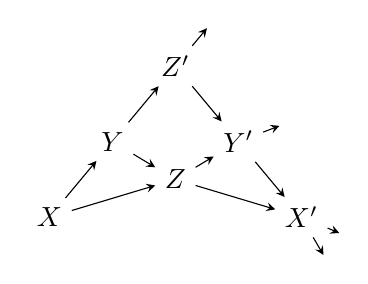
\begin{tikzpicture}[>=stealth,scale=.8]
\node(a)at(0,0){$X$};\node(b)at(1,1.2){$Y$};\node(c)at(2,2.4){$Z'$};\node(d)at(2,.6){$Z$};\node(e)at(3,1.2){$Y'$};\node(f)at(4,0){$X'$};
\draw[->](a)--(b);\draw[->](b)--(c);\draw[->](c)--(e);\draw[->](e)--(f);\draw[->](a)--(d);\draw[->](b)--(d);\draw[->](d)--(e);\draw[->](d)--(f);
\draw[->](c)--++(.5,.6);\draw[->](e)--++(.65,.25);\draw[->](f)--++(.6,-.25);\draw[->](f)--++(.35,-.6);
\end{tikzpicture}
\tag{1.1.7.1}
\end{equation*}
这一画法突出了\term{distinguished-triangle}{区别三角}的态射
\[
 (X,Y,Z')\longrightarrow(X,Z,Y')\longrightarrow(Y,Z,X')\longrightarrow(Z',Y',X'),
\]
只是对每个态射，其中一个相应的交换方形没有明显显示出来。此外，图中的对称性也被打破了，所以补全上述态射链的\term{distinguished-triangle}{区别三角}态射 $(Z',Y',X')\to(Z',X[1],Y[1])$ 没有明显显示出来。

\par\medskip\noindent\textbf{1.1.8.} 可将(1.1.7.1)与如下事实比较：在\term{abelian-category}{阿贝尔范畴}中，两个可复合单态射 $X\to Y\to Z$ 给出由短\term{exact-sequence}{正合列}组成的图
\SourcePage{30}
\begin{equation*}
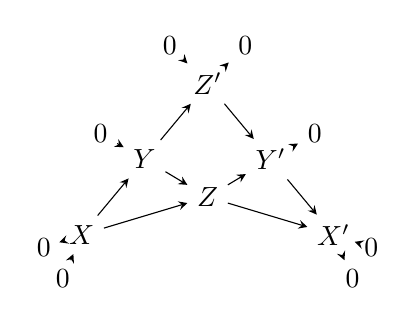
\begin{tikzpicture}[>=stealth,scale=.8]
\node(a)at(0,0){$X$};\node(b)at(1,1.2){$Y$};\node(c)at(2,2.4){$Z'$};\node(d)at(2,.6){$Z$};\node(e)at(3,1.2){$Y'$};\node(f)at(4,0){$X'$};
\draw[->](a)--(b);\draw[->](b)--(c);\draw[->](c)--(e);\draw[->](e)--(f);\draw[->](a)--(d);\draw[->](b)--(d);\draw[->](d)--(e);\draw[->](d)--(f);
\node(z1)at(-.6,-.2){$0$};\draw[->](z1)--(a);\node(z2)at(-.3,-.7){$0$};\draw[->](z2)--(a);
\node(z3)at(.3,1.6){$0$};\draw[->](z3)--(b);\node(z4)at(1.4,3){$0$};\draw[->](z4)--(c);
\node(z5)at(2.6,3){$0$};\draw[->](c)--(z5);\node(z6)at(3.7,1.6){$0$};\draw[->](e)--(z6);
\node(z7)at(4.6,-.2){$0$};\draw[->](f)--(z7);\node(z8)at(4.3,-.7){$0$};\draw[->](f)--(z8);
\end{tikzpicture}\tag{1.1.8.1}
\end{equation*}
它表达的是 $(Z/X)/(Y/X)=Z/Y$。(1.1.7.1)与(1.1.8.1)的关系如下。设在 $A$ 中对象的\term{complex}{复形}所成的\term{abelian-category}{阿贝尔范畴} $C(A)$ 中给定一个图(1.1.8.1)。$C(A)$ 中每个短\term{exact-sequence}{正合列}都定义 $D(A)$ 中的一个\term{distinguished-triangle}{区别三角}（[10] 第31页）；由图(1.1.8.1)的短\term{exact-sequence}{正合列}得到的\term{distinguished-triangle}{区别三角}构成一个八面体(1.1.7.1)。特别地，通过 $A\mapsto(\text{仅在0次为 $A$ 的\term{complex}{复形}})$，将\term{abelian-category}{阿贝尔范畴} $A$ 与 $DA$ 的一个全子范畴等同。于是对 $A$ 中任意短\term{exact-sequence}{正合列} $0\to A\to B\to C\to0$，都存在唯一的从 $C$ 到 $A$ 的一次箭头 $d$，使三角 $A\to B\to C\xrightarrow{d}$ 为\term{distinguished-triangle}{区别三角}。存在性是每个\term{complex}{复形}短\term{exact-sequence}{正合列}都确定\term{distinguished-triangle}{区别三角}（[10] 第31页）的特例；唯一性来自下述1.1.10以及：当 $A,B$ 属于 $A$ 时，$n<0$ 蕴涵 $\Hom^n(A,B)=0$（$n\geq0$ 时，它是 $A$ 被 $B$ \term{extension}{扩张}的第 $n$ 个 Yoneda $\Ext$）。从 $A$ 中的图(1.1.8.1)出发，在 $DA$ 中将其中每个短\term{exact-sequence}{正合列}补成\term{distinguished-triangle}{区别三角}，就得到图(1.1.7.1)。这是 TR 4 的一个推论。

\par\medskip\noindent\textbf{命题1.1.9。} 设 $(X,Y,Z)$ 与 $(X',Y',Z')$ 是两个\term{distinguished-triangle}{区别三角}，$g:Y\to Y'$：
\[
\begin{tikzcd}[ampersand replacement=\&]
X\arrow[r,"{u}"]\arrow[d,dashed,"{f}"']\&Y\arrow[r,"{v}"]\arrow[d,"{g}"]\&Z\arrow[r,"{d}"]\arrow[d,dashed,"{h}"]\&X[1]\\
X'\arrow[r,"{u'}"']\&Y'\arrow[r,"{v'}"']\&Z'\arrow[r,"{d'}"']\&X'[1]
\end{tikzcd}
\]
以下条件\term{equivalence}{等价}：\textup{(a)} $v'gu=0$；\textup{(b)} 存在 $f$ 使第一个方形交换；\textup{(b$'$)} 存在 $h$ 使第二个方形交换；\textup{(c)} 存在三角态射 $(f,g,h)$。若这些条件成立且 $\Hom^{-1}(X,Z')=0$，则 \textup{(b)} 中的 $f$ 和 \textup{(b$'$)} 中的 $h$ 各自唯一。

将\term{exact-sequence}{正合列}
\[
 \Hom^{-1}(X,Z')\longrightarrow\Hom(X,X')\longrightarrow\Hom(X,Y')\longrightarrow\Hom(X,Z')
\]
应用于 $\Hom(X,Y')$ 中的 $gu$，便得 $(a)\Longleftrightarrow(b)$，并且当 $\Hom^{-1}(X,Z')=0$ 时 $f$ 唯一。$(b)\Longrightarrow(c)$ 来自 TR 2：若 $f$ 满足 $(b)$，则存在 $h$ 使
\SourcePage{31}
$(f,g,h)$ 成为三角态射。反向蕴涵显然。最后，\term{duality}{对偶}论证给出 $(a)\Longleftrightarrow(b')$，以及当 $\Hom^{-1}(X,Z')=0$ 时 $h$ 的唯一性。

\par\medskip\noindent\textbf{推论1.1.10。} 设 $X\xrightarrow{u}Y\xrightarrow{v}Z\xrightarrow{d}$ 是\term{distinguished-triangle}{区别三角}。若 $\Hom^{-1}(X,Z)=0$，则
\begin{enumerate}[label=(\roman*)]
\item $u$ 的\term{cone}{锥}在唯一同构意义下唯一；
\item $d$ 是唯一使 $X\xrightarrow{u}Y\xrightarrow{v}Z\xrightarrow{x}$ 为\term{distinguished-triangle}{区别三角}的态射 $x:Z\to X[1]$。
\end{enumerate}
若在1.1.9中取 $X=X'$、$Y=Y'$，并令 $f,g$ 都是恒等态射，则 $Z\simeq Z'$，从而 $\Hom^{-1}(X,Z')=0$；于是(i)来自 $h$ 的唯一性。为证(ii)，将1.1.9应用于
\[
\begin{tikzcd}[ampersand replacement=\&]
X\arrow[r,"{u}"]\arrow[d,equal]\&Y\arrow[r,"{v}"]\arrow[d,equal]\&Z\arrow[r,"{d}"]\arrow[d,dashed,"{h}"]\&X[1]\arrow[d,equal]\\
X\arrow[r,"{u}"']\&Y\arrow[r,"{v}"']\&Z\arrow[r,"{x}"']\&X[1]
\end{tikzcd}
\]
必有 $h=\id_Z$，故 $d=x$。

\term{duality}{对偶}地，在1.1.10的条件下，$v$ 的\term{cone}{锥}在唯一同构意义下唯一。

下面的命题由 J. L. Verdier 告知我们。

\par\medskip\noindent\textbf{命题1.1.11。} 任意交换方形 $(X'Y'XY)$ 都可以补成一个九对象图：
\[
\begin{tikzcd}[ampersand replacement=\&,column sep=small]
X'[1]\arrow[r,dashed]\&Y'[1]\arrow[r,dashed]\&Z'[1]\arrow[r,dashed]\&X'[2]\\
X''\arrow[u,dashed]\arrow[r]\&Y''\arrow[u,dashed]\arrow[r]\&Z''\arrow[u,dashed]\arrow[r]\&X''[1]\arrow[u,dashed]\\
X\arrow[u]\arrow[r]\&Y\arrow[u]\arrow[r]\&Z\arrow[u]\arrow[r]\&X[1]\arrow[u,dashed]\\
X'\arrow[u]\arrow[r]\&Y'\arrow[u]\arrow[r]\&Z'\arrow[u]\arrow[r]\&X'[1]\arrow[u,dashed]
\end{tikzcd}
\]
其中虚线箭头由实线箭头施以\term{shift-functor}{平移函子}得到；各方形交换，唯独右上角的方形反交换；实线的各行、各列都是\term{distinguished-triangle}{区别三角}。

取\term{distinguished-triangle}{区别三角} $(X',Y',Z')$、$(X,Y,Z)$、$(X',X,X'')$、$(Y',Y,Y'')$ 和 $(X',Y,A)$，其底边分别为所给交换方形的四边及其对角线 $X'\to Y$。公理 TR 4 允许我们补全如下两个八面体：
\SourcePage{32}
\begin{center}
\begin{tikzpicture}[>=stealth,scale=.68]
\node(a)at(0,0){$X'$};\node(b)at(1,1.2){$Y'$};\node(c)at(2,2.4){$Z'$};\node(d)at(2,.6){$Y$};\node(e)at(3,1.2){$A$};\node(f)at(4,0){$Y''$};
\draw[->](a)--(b);\draw[->](b)--(c);\draw[->](c)--(e);\draw[->](e)--(f);\draw[->](a)--(d);\draw[->](b)--(d);\draw[->](d)--(e);\draw[->](d)--(f);\draw[->](c)--++(.4,.6);\draw[->](e)--++(.6,.2);\draw[->](f)--++(.5,-.25);\draw[->](f)--++(.3,-.6);
\node at(-.5,1.2){(1)};\node at(2,-.8){基于 $X'\to Y'\to Y$};
\begin{scope}[xshift=6.4cm]
\node(a)at(0,0){$X'$};\node(b)at(1,1.2){$X$};\node(c)at(2,2.4){$X''$};\node(d)at(2,.6){$Y$};\node(e)at(3,1.2){$A$};\node(f)at(4,0){$Z$};
\draw[->](a)--(b);\draw[->](b)--(c);\draw[->](c)--(e);\draw[->](e)--(f);\draw[->](a)--(d);\draw[->](b)--(d);\draw[->](d)--(e);\draw[->](d)--(f);\draw[->](c)--++(.4,.6);\draw[->](e)--++(.6,.2);\draw[->](f)--++(.5,-.25);\draw[->](f)--++(.3,-.6);
\node at(-.5,1.2){(2)};\node at(2,-.8){基于 $X'\to X\to Y$};
\end{scope}
\end{tikzpicture}
\end{center}
再补出八面体
\begin{center}
\begin{tikzpicture}[>=stealth,scale=.7]
\node(a)at(0,0){$X''$};\node(b)at(1,1.2){$A$};\node(c)at(2,2.4){$Z$};\node(d)at(2,.6){$Y''$};\node(e)at(3,1.2){$Z''$};\node(f)at(4,0){$Z'[1]$};
\draw[->](a)--(b);\draw[->](b)--(c);\draw[->](c)--(e);\draw[->](e)--(f);\draw[->](a)--(d);\draw[->](b)--(d);\draw[->](d)--(e);\draw[->](d)--(f);\draw[->](c)--++(.4,.6);\draw[->](e)--++(.6,.2);\draw[->](f)--++(.5,-.25);\draw[->](f)--++(.3,-.6);
\node at(-.6,1.2){(3)};\node at(2,-.8){基于 $X''\to A\to Y''$};
\end{tikzpicture}
\end{center}
其中的\term{distinguished-triangle}{区别三角} $(A,Y'',Z'[1])$ 由(1)中的 $(Z',A,Y'')$ 旋转而得：将箭头 $Z'\to A$ 改变符号。

所需的\term{distinguished-triangle}{区别三角}都出现在这些八面体中，只有 $(Z',Z,Z'')$ 以 $(Z,Z'',Z'[1])$ 的形式出现；将箭头 $Z'\to Z$ 改变符号，就可由 $(Z,Z'',Z'[1])$ 得到 $(Z',Z,Z'')$。

为证明所需的交换性与反交换性，注意从 $X',Y',Z'$ 到 $X,Y,Z$ 的箭头组成如下三角态射的复合：
\[
 (X',Y',Z')\xrightarrow{(1)}(X',Y,A)\xrightarrow{(2)}(X,Y,Z),
\]
这些态射出现在(1)与(2)中；从 $X,Y,Z$ 到 $X'',Y'',Z''$ 的箭头组成如下三角态射的复合：
\[
 (X,Y,Z)\xrightarrow{(2)}(X'',A,Z)\xrightarrow{(3)}(X'',Y'',Z'');
\]
而从 $X'',Y'',Z''$ 到 $X'[1],Y'[1],Z'[1]$ 的箭头组成如下三角态射的复合：
\[
 (X'',Y'',Z'')\xrightarrow{(3)}(A,Y'',Z'[1])\xrightarrow{(1)}(X'[1],Y'[1],Z'[1]),
\]
最后一个箭头由(1)中的三角态射 $(Z',A,Y'')\to(Z',X'[1],Y'[1])$ 旋转而来。在\term{distinguished-triangle}{区别三角} $(X'[1],Y'[1],Z'[1])$ 中，一次箭头与三角 $(X',Y',Z')$ 的一次箭头的平移相差一个符号；这就解释了第九个方形的反交换性。

\par\medskip\noindent\textbf{注1.1.12。} 一个由\term{complex}{复形}\term{exact-sequence}{正合列}组成的方形，在\term{derived-category}{导出范畴}中定义一个九对象图。第九个方形的反交换性精确说明了相应连接同态的反交换性。

\par\medskip\noindent\textbf{注1.1.13。} 在通常的\term{triangulated-category}{三角范畴}中（$A$ 加性时的 $KA$，$A$ 正合时的 $DA$，稳定\term{homotopy}{同伦}范畴等），每个“八面体上半部”形式的图都能补成一个八面体，
\SourcePage{33}
使下列三角为\term{distinguished-triangle}{区别三角}：
\[
 Y\longrightarrow Y'\longrightarrow X'\oplus X[1]\xrightarrow{(1)}Y,
 \qquad
 Y\longrightarrow Z\oplus Z'\longrightarrow Y'\xrightarrow{(1)}Y
\]
（箭头取自八面体，唯独第一式中的 $Y'\to X[1]$、第二式中的 $Z'\to Y'$ 分别与八面体中的箭头反号）。一般情况下是否如此，我们并不清楚。如果这些三角今后有用，或许应该加强\term{triangulated-category}{三角范畴}的公理 TR 4，重新定义“八面体”，将上述三角为\term{distinguished-triangle}{区别三角}纳入八面体的定义。

\par\medskip\noindent\textbf{注1.1.14。} 三角图与八面体图有如下推广；它们分别是 $N=3$ 与 $N=4$ 的特例。对 $N\geq2$，一个这样的图包含以下数据：
\begin{enumerate}[label=(\alph*)]
\item 对 $\Z$ 的每个满足 $0<\#I<N$ 的区间 $I$，给定对象 $K(I)$。
\item 若 $I=[a,b[$、$J=[c,d[$，定义 $I\leq J\Longleftrightarrow(a\leq c\text{ 且 }b\leq d)$。对 $I\leq J$ 给定箭头 $\varphi_{JI}:K(I)\to K(J)$，满足 $\varphi_{KJ}\varphi_{JI}=\varphi_{KI}$ 及 $\varphi_{II}=\id$。若 $I=[a,b[$、$J=[c,d[$ 且 $b\leq c$，则要求 $\varphi_{JI}=0$。
\item 对 $I=[a,b[$ 定义 $I^*=[b,a+N[$。给定同构 $K(I^*)=K(I)[1]$，对 $I\leq J$，使图
\[
\begin{tikzcd}[ampersand replacement=\&]
 K(I)[1]\arrow[r,equal]\arrow[d,"{\varphi_{JI}[1]}"']\&K(I^*)\arrow[d,"{\varphi_{J^*I^*}}"]\\
 K(J)[1]\arrow[r,equal]\&K(J^*)
\end{tikzcd}
\]
交换。
\item 对 $a<b<c<a+N$，由箭头 $\varphi$ 组成的三角
\[
 K([a,b[)\longrightarrow K([a,c[)\longrightarrow K([b,c[)\longrightarrow K([b,a+N[)=K([a,b[)[1]
\]
为\term{distinguished-triangle}{区别三角}。
\end{enumerate}
一个具有 $N-1$ 阶\term{filtration}{滤过}、且\term{filtration}{滤过}逐次可裂的\term{complex}{复形}，在 $KA$ 中定义这样的图。若 $K$ 的\term{filtration}{滤过} $W$ 取为递增\term{filtration}{滤过}，$W_0K=0$ 且 $W_{N-1}K=K$（即 $i\notin[1,N-1]$ 时 $\mathrm{Gr}^W_iK=0$），那么对 $1\leq a<b\leq N$ 有 $K([a,b[)=W_{b-1}K/W_{a-1}K$，并且 $K(\{0\})=K[-1]$。
\SourcePage{34}
\section*{1.2. 阿贝尔子范畴}
\addcontentsline{toc}{section}{1.2. 阿贝尔子范畴}
\par\medskip\noindent\textbf{1.2.0.} 设 $\mathcal D$ 是\term{triangulated-category}{三角范畴}，$\mathcal C$ 是 $\mathcal D$ 的全子范畴。我们假设，当 $i<0$ 且 $X,Y\in\mathcal C$ 时，$\Hom^i(X,Y):=\Hom(X,Y[i])=0$。

\par\medskip\noindent\textbf{例1.2.1。} $\mathcal D$ 是\term{abelian-category}{阿贝尔范畴} $A$ 的\term{derived-category}{导出范畴}，$\mathcal C=A$，并通过函子 $A\mapsto(\text{仅在0次为 $A$ 的\term{complex}{复形}})$ 将它与 $\mathcal D$ 的全子范畴等同。

\par\medskip\noindent\textbf{命题1.2.2。} 设 $f:X\to Y$ 是 $\mathcal C$ 中的态射。将 $f$ 补成\term{distinguished-triangle}{区别三角} $X\to Y\to S\to$，并假设 $S$ 属于一个\term{distinguished-triangle}{区别三角} $N[1]\to S\to C\to$，其中 $N,C\in\mathcal C$：
\begin{equation*}
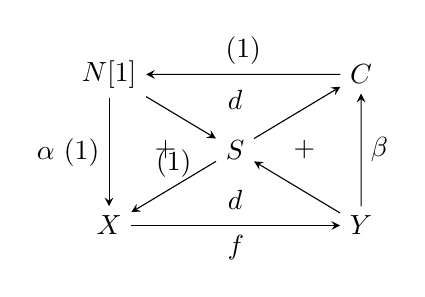
\begin{tikzpicture}[>=stealth,scale=.8]
\node(a)at(0,2.4){$N[1]$};\node(b)at(4,2.4){$C$};\node(c)at(0,0){$X$};\node(d)at(4,0){$Y$};\node(e)at(2,1.2){$S$};
\draw[->](b)--node[above]{$(1)$}(a);\draw[->](a)--node[left]{$\alpha\ (1)$}(c);\draw[->](c)--node[below]{$f$}(d);\draw[->](d)--node[right]{$\beta$}(b);
\draw[->](a)--(e);\draw[->](e)--(b);\draw[->](e)--node[above]{$(1)$}(c);\draw[->](d)--(e);
\node at(2,2){$d$};\node at(.9,1.2){$+$};\node at(3.1,1.2){$+$};\node at(2,.4){$d$};
\end{tikzpicture}\tag{1.2.2.1}
\end{equation*}
标有 $+$ 的三角交换，标有 $d$ 的三角为\term{distinguished-triangle}{区别三角}。则 $\alpha[-1]:N\to X$ 是 $f$ 在 $\mathcal C$ 中的核，$\beta:Y\to C$ 是其余核。

对 $Z\in\mathcal C$，由 $\Hom$ 的长\term{exact-sequence}{正合列}和1.2.0，得到\term{exact-sequence}{正合列}
\[
 \begin{gathered}
 0\to\Hom^{-1}(Z,S)\to\Hom(Z,X)\to\Hom(Z,Y),\\[3pt]
 0\to\Hom(Z,N)\to\Hom^{-1}(Z,S)\to0.
 \end{gathered}
\]
这说明 $(N,\alpha[-1])$ 是 $f$ 的核。\term{duality}{对偶}论证表明 $(C,\beta)$ 是余核。

\par\medskip\noindent\textbf{例。} 对 $A\subset D(A)$（例1.2.1），$f:X\to Y$ 的\term{cone}{锥} $S$ 是\term{complex}{复形} $X\xrightarrow{f}Y$（$X$ 在 $-1$ 次，$Y$ 在0次）。它有子\term{complex}{复形} $\Ker(f)[1]=H^{-1}(S)[1]$，而商\term{complex}{复形} $X/\Ker(f)\to Y$ \term{quasi-isomorphism}{拟同构}地映到置于0次的 $\Coker(f)=H^0(S)$。因此得到图(1.2.2.1)。

\par\medskip\noindent\textbf{1.2.3.} 若 $\mathcal C$ 中的态射 $f:X\to Y$ 是某个图(1.2.2.1)的底边，则称它为 $\mathcal C$-\term{admissible}{容许}态射；当 $\mathcal C$ 不致混淆时，简称\term{admissible}{容许}态射。若 $f$ 是单态射，由1.2.2得 $N=0$，从而 $S\simeq C$，(1.2.2.1)退化为\term{distinguished-triangle}{区别三角} $(X,Y,C)$。若 $f$ 是满态射，则 $C=0$，从而 $N[1]\simeq S$，(1.2.2.1)退化为\term{distinguished-triangle}{区别三角} $(N,X,Y)$。反之，对任意\term{distinguished-triangle}{区别三角} $X\xrightarrow{f}Y\xrightarrow{g}Z\xrightarrow{d}$，
\SourcePage{35}
若 $X,Y,Z\in\mathcal C$，则 $f,g$ 均\term{admissible}{容许}，$f$ 是 $g$ 的核，$g$ 是 $f$ 的余核。由1.2.0及1.1.10，$d$ 由 $f,g$ 确定。

若 $\mathcal C$ 中的列 $X\to Y\to Z$ 可由某个\term{distinguished-triangle}{区别三角}去掉一次箭头得到，则称它为\term{admissible}{容许}短\term{exact-sequence}{正合列}。

\par\medskip\noindent\textbf{命题1.2.4。} 假设 $\mathcal C$ 对有限直和封闭。以下条件\term{equivalence}{等价}：
\begin{enumerate}[label=(\roman*)]
\item $\mathcal C$ 是\term{abelian-category}{阿贝尔范畴}，且它的短\term{exact-sequence}{正合列}均\term{admissible}{容许}；
\item $\mathcal C$ 的每个态射都是 $\mathcal C$-\term{admissible}{容许}态射。
\end{enumerate}
证明 $(ii)\Longrightarrow(i)$。由1.2.2，$\mathcal C$ 的每个态射都有核与余核；要证 $\mathcal C$ 是\term{abelian-category}{阿贝尔范畴}，只须再验证 $\mathrm{Coim}(f)\simeq\im(f)$。将(1.2.2.1)看作八面体的下半部，应用 TR $4'$（见1.1.7）补成八面体：
\begin{center}
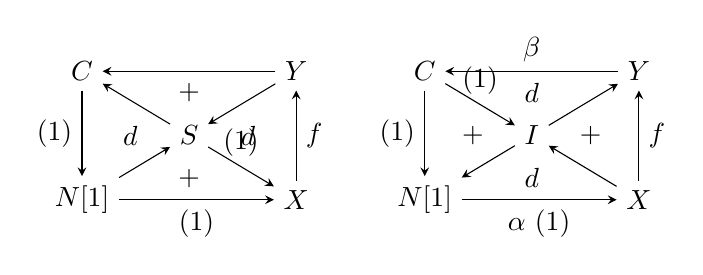
\begin{tikzpicture}[>=stealth,scale=.68]
\node(a)at(0,2.4){$C$};\node(b)at(4,2.4){$Y$};\node(c)at(0,0){$N[1]$};\node(d)at(4,0){$X$};\node(e)at(2,1.2){$S$};
\draw[->](b)--(a);\draw[->](a)--node[left]{$(1)$}(c);\draw[->](c)--node[below]{$(1)$}(d);\draw[->](d)--node[right]{$f$}(b);\draw[->](e)--(a);\draw[->](b)--(e);\draw[->](c)--(e);\draw[->](e)--node[above]{$(1)$}(d);\node at(2,2){$+$};\node at(.9,1.2){$d$};\node at(3.1,1.2){$d$};\node at(2,.4){$+$};
\begin{scope}[xshift=6.4cm]
\node(a)at(0,2.4){$C$};\node(b)at(4,2.4){$Y$};\node(c)at(0,0){$N[1]$};\node(d)at(4,0){$X$};\node(e)at(2,1.2){$I$};
\draw[->](b)--node[above]{$\beta$}(a);\draw[->](a)--node[left]{$(1)$}(c);\draw[->](c)--node[below]{$\alpha\ (1)$}(d);\draw[->](d)--node[right]{$f$}(b);\draw[->](a)--node[above]{$(1)$}(e);\draw[->](e)--(b);\draw[->](e)--(c);\draw[->](d)--(e);\node at(2,2){$d$};\node at(.9,1.2){$+$};\node at(3.1,1.2){$+$};\node at(2,.4){$d$};
\end{scope}
\end{tikzpicture}
\end{center}
由1.2.2，$\beta$ 作为 $f$ 的余核，是满态射。由1.2.3及\term{distinguished-triangle}{区别三角} $(I,Y,C)$，知 $I\in\mathcal C$ 且 $I$ 是 $f$ 的像。\term{duality}{对偶}地，将上半部的另一个\term{distinguished-triangle}{区别三角}旋转所得的\term{distinguished-triangle}{区别三角} $(N,X,I)$ 表明，$I$ 是 $f$ 的余像。最后，由1.2.3，$\mathcal C$ 的短\term{exact-sequence}{正合列}均\term{admissible}{容许}。

证明 $(i)\Longrightarrow(ii)$。$f:X\to Y$ 的核 $N$、余核 $C$ 和像 $I$ 给出两个短\term{exact-sequence}{正合列} $0\to N\to X\to I\to0$ 与 $0\to I\to Y\to C\to0$，因而给出组成上述上半部图的两个三角。应用 TR 4，便得到下半部，即 $f$ \term{admissible}{容许}。

\par\medskip\noindent\textbf{定义1.2.5。} $\mathcal D$ 的全子范畴 $\mathcal C$ 若满足1.2.0及1.2.4的\term{equivalence}{等价}条件，则称为\term{admissible}{容许}\term{abelian-subcategory}{阿贝尔子范畴}。

\par\medskip\noindent\textbf{1.2.6.} 在\term{triangulated-category}{三角范畴} $\mathcal D$ 中，若存在\term{distinguished-triangle}{区别三角} $(X,Y,Z)$，有时称对象 $Y$ 是 $Z$ 被 $X$ 的\term{extension}{扩张}。若对每个满足 $X,Z\in\mathcal D'$ 的\term{distinguished-triangle}{区别三角} $(X,Y,Z)$ 都有 $Y\in\mathcal D'$，则称 $\mathcal D$ 的子范畴 $\mathcal D'$ 对\term{extension}{扩张}封闭。

\SourcePage{36}
\section*{1.3. $t$-范畴}
\addcontentsline{toc}{section}{1.3. $t$-范畴}
\par\medskip\noindent\textbf{定义1.3.1。} 一个 $t$-范畴是\term{triangulated-category}{三角范畴} $\mathcal D$，配备两个严格全子范畴 $\mathcal D^{\leq0}$ 与 $\mathcal D^{\geq0}$，使得置 $\mathcal D^{\leq n}:=\mathcal D^{\leq0}[-n]$、$\mathcal D^{\geq n}:=\mathcal D^{\geq0}[-n]$ 后，有：
\begin{enumerate}[label=(\roman*)]
\item 当 $X\in\mathcal D^{\leq0}$、$Y\in\mathcal D^{\geq1}$ 时，$\Hom(X,Y)=0$；
\item $\mathcal D^{\leq0}\subset\mathcal D^{\leq1}$ 且 $\mathcal D^{\geq0}\supset\mathcal D^{\geq1}$；
\item 对任意 $X\in\mathcal D$，存在\term{distinguished-triangle}{区别三角} $(A,X,B)$，其中 $A\in\mathcal D^{\leq0}$、$B\in\mathcal D^{\geq1}$。
\end{enumerate}
也称 $(\mathcal D^{\leq0},\mathcal D^{\geq0})$ 为 $\mathcal D$ 上的一个\term{t-structure}{$t$-结构}。它的\term{heart}{心}是全子范畴 $\mathcal C:=\mathcal D^{\leq0}\cap\mathcal D^{\geq0}$。

\par\medskip\noindent\textbf{例1.3.2。} (i) 设 $A$ 是\term{abelian-category}{阿贝尔范畴}。$DA$ 的自然 \term{t-structure}{$t$-结构}定义为：$(DA)^{\leq n}$（相应地，$(DA)^{\geq n}$）是满足 $i>n$（相应地，$i<n$）时 $H^iK=0$ 的\term{complex}{复形} $K$ 所成的子范畴；也就是说，$K$ \term{quasi-isomorphism}{拟同构}于在次数 $>n$（相应地，$<n$）为零的\term{complex}{复形} $K'$。来验证1.3.1(iii)。对每个\term{complex}{复形} $K$，其\term{truncation}{截断} $\tau_{\leq0}K$ 是 $K$ 的子\term{complex}{复形} $\cdots\to K^{-1}\to\Ker(d^0)\to0\to\cdots$。须注意，[7] 将该\term{truncation}{截断}记为 $\sigma_{\leq0}K$，[8] 则记为 $t_{0]}$。置 $\tau_{\geq1}K:=K/\tau_{\leq0}K$，则 $\tau_{\leq0}K\in(DA)^{\leq0}$、$\tau_{\geq1}K\in(DA)^{\geq1}$；短\term{exact-sequence}{正合列} $0\to\tau_{\leq0}K\to K\to\tau_{\geq1}K\to0$ 给出所需的三角。1.3.1(i)、(ii)的验证留给读者。

(ii) 若 $(\mathcal D^{\leq0},\mathcal D^{\geq0})$ 是 $\mathcal D$ 上的 \term{t-structure}{$t$-结构}，则对任意整数 $n$，$(\mathcal D^{\leq n},\mathcal D^{\geq n})$ 也是一个 \term{t-structure}{$t$-结构}，称其由原 \term{t-structure}{$t$-结构}经平移得到。

(iii) 若 $(\mathcal D^{\leq0},\mathcal D^{\geq0})$ 是 $\mathcal D$ 上的 \term{t-structure}{$t$-结构}，则 $((\mathcal D^{\geq0})^{\mathrm{opp}},(\mathcal D^{\leq0})^{\mathrm{opp}})$ 是\term{duality}{对偶}\term{triangulated-category}{三角范畴} $\mathcal D^{\mathrm{opp}}$ 上的 \term{t-structure}{$t$-结构}，称为\term{duality}{对偶} \term{t-structure}{$t$-结构}。这使我们可以使用\term{duality}{对偶}论证（若将一个命题应用于\term{duality}{对偶} $t$-范畴得到另一个命题，就称二者\term{duality}{对偶}）。

以下设 $\mathcal D$ 是一个 $t$-范畴。

\par\medskip\noindent\textbf{命题1.3.3。} (i) 包含函子 $\mathcal D^{\leq n}\hookrightarrow\mathcal D$ 有右\term{adjunction}{伴随} $\tau_{\leq n}$，而 $\mathcal D^{\geq n}\hookrightarrow\mathcal D$ 有左\term{adjunction}{伴随} $\tau_{\geq n}$。

(ii) 对任意 $X\in\mathcal D$，存在唯一的态射 $d\in\Hom^1(\tau_{\geq1}X,\tau_{\leq0}X)$，使三角
\[
 \tau_{\leq0}X\longrightarrow X\longrightarrow\tau_{\geq1}X\xrightarrow{d}
\]
\SourcePage{37}
为\term{distinguished-triangle}{区别三角}。在唯一同构意义下，它是唯一满足 $A\in\mathcal D^{\leq0}$、$B\in\mathcal D^{\geq1}$ 的\term{distinguished-triangle}{区别三角} $(A,X,B)$。

由\term{duality}{对偶}性和平移，只须对 $\mathcal D^{\leq0}$ 验证(i)。也就是对每个 $X\in\mathcal D$，寻找 $A\in\mathcal D^{\leq0}$ 及箭头 $A\to X$（即 $\tau_{\leq0}$ 在 $X$ 处的值），使对任意 $T\in\mathcal D^{\leq0}$ 都有 $\Hom(T,A)\xrightarrow{\sim}\Hom(T,X)$。取1.3.1(iii)中的三角 $(A,X,B)$。$\Hom$ 的长\term{exact-sequence}{正合列}和条件1.3.1(i)、(ii)给出 $\Hom(T,A)\xrightarrow{\sim}\Hom(T,X)$，因此 $A=\tau_{\leq0}X$。这证明了(i)，也证明了\term{distinguished-triangle}{区别三角} $(\tau_{\leq0}X,X,\tau_{\geq1}X)$ 的存在性，以及：忘掉一次箭头后，1.3.1(iii)中的每个\term{distinguished-triangle}{区别三角} $(A,X,B)$ 都与此三角唯一同构。一次箭头的唯一性由1.3.1(i)、(ii)及1.1.10(ii)得到。

\par\medskip\noindent\textbf{1.3.4.} \term{distinguished-triangle}{区别三角} $(\tau_{\leq0}X,X,\tau_{\geq1}X)$ 表明下列条件\term{equivalence}{等价}：
\begin{align*}
 (a)\;&\tau_{\leq0}X=0,
 & (a')\;&\text{对每个 $T\in\mathcal D^{\leq0}$，$\Hom(T,X)=0$};\\
 (b)\;&X\xrightarrow{\sim}\tau_{\geq1}X,
 & (b')\;&X\in\mathcal D^{\geq1}.
\end{align*}
\term{equivalence}{等价}关系 $(a')\Longleftrightarrow(b')$ 可表述为：$\mathcal D^{\geq1}$ 是 $\mathcal D^{\leq0}$ 的右正交。由此可见，$\mathcal D^{\geq1}$ 对\term{extension}{扩张}封闭（1.2.6）。\term{duality}{对偶}地，$\tau_{\geq1}X=0$ 当且仅当 $X\in\mathcal D^{\leq0}$；$\mathcal D^{\leq0}$ 是 $\mathcal D^{\geq1}$ 的左正交，并对\term{extension}{扩张}封闭。特别地，$\mathcal D^{\leq0}$ 与 $\mathcal D^{\geq1}$ 都对有限直和封闭。

对 $a\leq b$，有 $\mathcal D^{\leq a}\subset\mathcal D^{\leq b}$，故存在唯一的态射 $\tau_{\leq a}X\to\tau_{\leq b}X$，使图
\[
\begin{tikzcd}[ampersand replacement=\&]
\tau_{\leq a}X\arrow[rr]\arrow[dr]\&\&\tau_{\leq b}X\arrow[dl]\\
\&X\&
\end{tikzcd}
\]
交换。它将 $\tau_{\leq a}X$ 与 $\tau_{\leq a}\tau_{\leq b}X$ 等同。\term{duality}{对偶}地，有态射 $\tau_{\geq a}X\to\tau_{\geq b}X$，将 $\tau_{\geq b}X$ 与 $\tau_{\geq b}\tau_{\geq a}X$ 等同。

对任意整数 $a$，记 $\tau_{>a}:=\tau_{\geq a+1}$、$\tau_{<a}:=\tau_{\leq a-1}$。由本段第一段平移可知，$X\in\mathcal D^{\leq a}$ \term{equivalence}{等价}于 $\tau_{>a}X=0$。设 $X\in\mathcal D^{\leq a}$。若 $b>a$，则 $\tau_{\geq b}X=0$；若 $b\leq a$，则 $\tau_{>a}\tau_{\geq b}X=\tau_{>a}X=0$。因此 $\tau_{\geq b}$ 将 $\mathcal D^{\leq a}$ 映入自身。

\par\medskip\noindent\textbf{命题1.3.5。} 设 $a\leq b$。对任意 $X\in\mathcal D$，存在唯一态射 $\tau_{\geq a}\tau_{\leq b}X\to\tau_{\leq b}\tau_{\geq a}X$，使图
\SourcePage{38}
\[
\begin{tikzcd}[ampersand replacement=\&]
 \tau_{\leq b}X\arrow[r]\arrow[d]\&X\arrow[r]\&\tau_{\geq a}X\\
 \tau_{\geq a}\tau_{\leq b}X\arrow[rr]\&\&\tau_{\leq b}\tau_{\geq a}X\arrow[u]
\end{tikzcd}
\]
交换。此态射是同构。

从 $\tau_{\leq b}X$ 到 $\tau_{\geq a}X\in\mathcal D^{\geq a}$ 的箭头唯一地经 $\tau_{\geq a}\tau_{\leq b}X$ 分解。因为 $\tau_{\geq a}\tau_{\leq b}X\in\mathcal D^{\leq b}$，该箭头又唯一地经 $\tau_{\leq b}\tau_{\geq a}X$ 分解。将 TR 4 应用于 $\tau_{<a}X\to\tau_{\leq b}X\to X$，得到八面体
\begin{equation*}
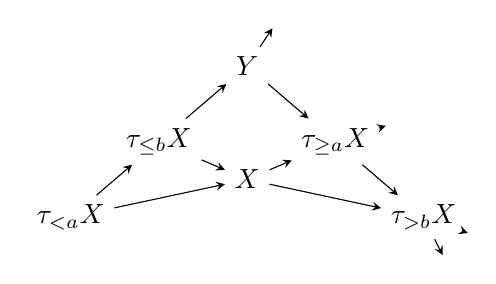
\begin{tikzpicture}[>=stealth,scale=.8]
\node(a)at(0,0){$\tau_{<a}X$};\node(b)at(1.4,1.2){$\tau_{\leq b}X$};\node(c)at(2.8,2.4){$Y$};\node(d)at(2.8,.6){$X$};\node(e)at(4.2,1.2){$\tau_{\geq a}X$};\node(f)at(5.6,0){$\tau_{>b}X$};
\draw[->](a)--(b);\draw[->](b)--(c);\draw[->](c)--(e);\draw[->](e)--(f);\draw[->](a)--(d);\draw[->](b)--(d);\draw[->](d)--(e);\draw[->](d)--(f);\draw[->](c)--++(.4,.6);\draw[->](e)--++(.8,.25);\draw[->](f)--++(.7,-.25);\draw[->](f)--++(.3,-.6);
\end{tikzpicture}\tag{1.3.5.1}
\end{equation*}
在这个八面体中，$Y$ 一方面是 $\tau_{\geq a}\tau_{\leq b}X$，这是因为\term{distinguished-triangle}{区别三角} $(\tau_{<a}X,\tau_{\leq b}X,Y)$ 中有 $\tau_{<a}X=\tau_{<a}\tau_{\leq b}X$；另一方面又是 $\tau_{\leq b}\tau_{\geq a}X$，这是因为有\term{distinguished-triangle}{区别三角} $(Y,\tau_{\geq a}X,\tau_{>b}X)$。

约定 $\tau_{[a,b]}X:=\tau_{\geq a}\tau_{\leq b}X\xrightarrow{\sim}\tau_{\leq b}\tau_{\geq a}X$。

\par\medskip\noindent\textbf{定理1.3.6。} $t$-范畴 $\mathcal D$ 的\term{heart}{心} $\mathcal C:=\mathcal D^{\leq0}\cap\mathcal D^{\geq0}$ 是 $\mathcal D$ 的\term{admissible}{容许}\term{abelian-subcategory}{阿贝尔子范畴}，并对\term{extension}{扩张}封闭（1.2.5、1.2.6）。函子 $H^0:=\tau_{\geq0}\tau_{\leq0}:\mathcal D\to\mathcal C$ 是\term{cohomological-functor}{上同调函子}。

\par\medskip\noindent\textbf{例。} 在1.3.2(i)的情形，$\mathcal C$ 是由与 $A$ 的某个对象同构的 $\mathcal D$ 中对象组成的范畴（这里使用 $A$ 到 $DA$ 的自然嵌入），$H^0$ 与通常的 $H^0$ 函子等同。

\par\medskip\noindent\textbf{证明。} 设 $X,Y\in\mathcal C$，$f:X\to Y$ 的\term{cone}{锥}为 $S$。\term{distinguished-triangle}{区别三角} $(Y,S,X[1])$ 表明 $S\in\mathcal D^{\leq0}\cap\mathcal D^{\geq-1}$。故\term{truncation}{截断} $\tau_{\geq0}S$ 与 $\tau_{\leq-1}S$ 分别属于 $\mathcal C$ 与 $\mathcal C[1]$；\term{distinguished-triangle}{区别三角} $(\tau_{\leq-1}S,S,\tau_{\geq0}S)$ 给出图(1.2.2.1)。这证明 $\mathcal C$ 是\term{admissible}{容许}\term{abelian-subcategory}{阿贝尔子范畴}。$\mathcal C$ 对\term{extension}{扩张}封闭由1.3.4得到。

还须证明：对每个\term{distinguished-triangle}{区别三角} $(X,Y,Z)$，列 $H^0X\to H^0Y\to H^0Z$ 正合。
\SourcePage{39}
\noindent\textbf{情形1。} 若 $X,Y,Z\in\mathcal D^{\leq0}$，则列 $H^0X\to H^0Y\to H^0Z\to0$ 正合。

对 $U\in\mathcal D^{\leq0}$、$V\in\mathcal D^{\geq0}$，有 $H^0U=\tau_{\geq0}U$、$H^0V=\tau_{\leq0}V$，以及
\[
 \Hom(H^0U,H^0V)\xrightarrow{\sim}\Hom(U,H^0V)\xrightarrow{\sim}\Hom(U,V).
\]
对 $T\in\mathcal C$（故 $T\in\mathcal D^{\geq0}$），$\Hom$ 的长\term{exact-sequence}{正合列}给出
\[
 0\to\Hom(Z,T)\to\Hom(Y,T)\to\Hom(X,T),
\]
即 $0\to\Hom(H^0Z,T)\to\Hom(H^0Y,T)\to\Hom(H^0X,T)$。这对每个 $T$ 都成立，因而得到所需正合性。

\noindent\textbf{情形2。} 若 $X\in\mathcal D^{\leq0}$，则列 $H^0X\to H^0Y\to H^0Z\to0$ 正合。

对 $T\in\mathcal D^{\geq1}$，$\Hom$ 的长\term{exact-sequence}{正合列}给出 $\Hom(Z,T)\xrightarrow{\sim}\Hom(Y,T)$，因此 $\tau_{\geq1}Y\xrightarrow{\sim}\tau_{\geq1}Z$。将 TR $4'$（见1.1.7）应用于 $Y\to Z\to\tau_{\geq1}Z$（也可以将 TR 4 应用于 $X\to\tau_{\leq0}Y\to Y$）：
\begin{center}
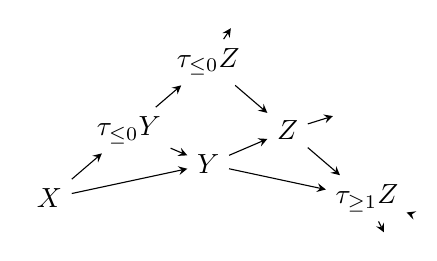
\begin{tikzpicture}[>=stealth,scale=.72]
\node(a)at(0,0){$X$};\node(b)at(1.4,1.2){$\tau_{\leq0}Y$};\node(c)at(2.8,2.4){$\tau_{\leq0}Z$};\node(d)at(2.8,.6){$Y$};\node(e)at(4.2,1.2){$Z$};\node(f)at(5.6,0){$\tau_{\geq1}Z$};
\draw[->](a)--(b);\draw[->](b)--(c);\draw[->](c)--(e);\draw[->](e)--(f);\draw[->](a)--(d);\draw[->](b)--(d);\draw[->](d)--(e);\draw[->](d)--(f);\draw[->](c)--++(.4,.6);\draw[->](e)--++(.8,.25);\draw[->](f)--++(.7,-.25);\draw[->](f)--++(.3,-.6);
\end{tikzpicture}
\end{center}
便得到\term{distinguished-triangle}{区别三角} $(X,\tau_{\leq0}Y,\tau_{\leq0}Z)$，可应用情形1。

\noindent\textbf{情形 $2^*$。} \term{duality}{对偶}地，若 $Z\in\mathcal D^{\geq0}$，则列 $0\to H^0X\to H^0Y\to H^0Z$ 正合。

\noindent\textbf{一般情形。} TR 4 给出八面体
\begin{center}
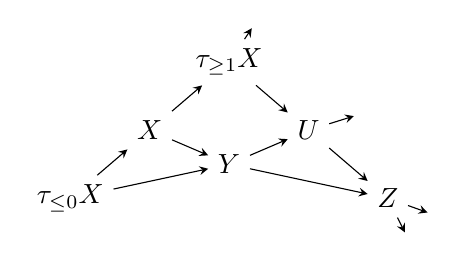
\begin{tikzpicture}[>=stealth,scale=.72]
\node(a)at(0,0){$\tau_{\leq0}X$};\node(b)at(1.4,1.2){$X$};\node(c)at(2.8,2.4){$\tau_{\geq1}X$};\node(d)at(2.8,.6){$Y$};\node(e)at(4.2,1.2){$U$};\node(f)at(5.6,0){$Z$};
\draw[->](a)--(b);\draw[->](b)--(c);\draw[->](c)--(e);\draw[->](e)--(f);\draw[->](a)--(d);\draw[->](b)--(d);\draw[->](d)--(e);\draw[->](d)--(f);\draw[->](c)--++(.4,.6);\draw[->](e)--++(.8,.25);\draw[->](f)--++(.7,-.25);\draw[->](f)--++(.3,-.6);
\end{tikzpicture}
\end{center}
将情形2应用于 $(\tau_{\leq0}X,Y,U)$，得到\term{exact-sequence}{正合列} $H^0X\to H^0Y\to H^0U\to0$；将情形 $2^*$ 应用于 $(U,Z,(\tau_{\geq1}X)[1])$，得到 $0\to H^0U\to H^0Z$。由此可得 $H^0X\to H^0Y\to H^0Z$ 正合。

若 $\bigcap_n\mathcal D^{\leq n}$ 与 $\bigcap_n\mathcal D^{\geq n}$ 都只含零对象，则称该 \term{t-structure}{$t$-结构}\term{nondegenerate}{非退化}。置 $H^iX:=H^0(X[i])$。

\par\medskip\noindent\textbf{命题1.3.7。} 若 $\mathcal D$ 的 \term{t-structure}{$t$-结构}\term{nondegenerate}{非退化}，则函子族 $H^i$ 是\term{conservative}{保守}的；而且，对 $X\in\mathcal D$，
\SourcePage{40}
$X\in\mathcal D^{\leq0}$（相应地，$X\in\mathcal D^{\geq0}$）当且仅当 $i>0$（相应地，$i<0$）时 $H^iX=0$。

设 $X\in\mathcal D$。先证明：若所有 $H^iX$ 都为零，则 $X=0$。若 $X\in\mathcal D^{\leq0}$，则 $H^0X=0$ 保证 $X\in\mathcal D^{\leq-1}$；继续下去可知 $X\in\bigcap_n\mathcal D^{\leq n}$，所以 $X=0$。\term{duality}{对偶}地，若 $X\in\mathcal D^{\geq0}$，同样有 $X=0$。一般情况下，$\tau_{\leq0}X$ 与 $\tau_{\geq1}X$ 的所有 $H^i$ 仍为零，故二者均为零；由\term{distinguished-triangle}{区别三角} $(\tau_{\leq0}X,X,\tau_{\geq1}X)$ 即得结论。

若\term{cone}{锥}为 $Z$ 的态射 $f:X\to Y$ 诱导同构 $H^i(X)\xrightarrow{\sim}H^i(Y)$，则\term{cohomology}{上同调}长\term{exact-sequence}{正合列}表明所有 $H^i(Z)$ 都为零。因此 $Z=0$，$f$ 是同构。最后，若 $i>0$ 时 $H^i(X)=0$，则所有 $H^i(\tau_{>0}X)$ 都为零，故 $\tau_{>0}X=0$，由1.3.4知 $X\in\mathcal D^{\leq0}$。$\mathcal D^{\geq0}$ 的结论由\term{duality}{对偶}性得到。

\par\medskip\noindent\textbf{1.3.8.} 定理1.3.6将 $\mathcal D$ 的每个 \term{t-structure}{$t$-结构}对应于一个\term{admissible}{容许}\term{abelian-subcategory}{阿贝尔子范畴} $\mathcal C$；它有一个逆命题，表述如下（1.3.9）。其证明将持续到1.3.14。本文后续部分不会使用这个结果。

\par\medskip\noindent\textbf{1.3.9.} 设 $\mathcal D$ 是\term{triangulated-category}{三角范畴}，$\operatorname{Isom}(\mathcal D)$ 是其对象的同构类集合，$X\in\mathcal D$ 的同构类记为 $[X]$。以 $*$ 表示如下运算，将 $\operatorname{Isom}(\mathcal D)$ 的两个子集对应于第三个子集：
\[
 A*B=\{[X]\mid\text{存在\term{distinguished-triangle}{区别三角} $(U,X,V)$，其中 $[U]\in A$、$[V]\in B$}\}.
\]
\par\medskip\noindent\textbf{引理1.3.10。} 运算 $*$ 满足结合律。

\noindent\textbf{证明。} 只须证明，对 $X,Y,Z\in\mathcal D$ 有
\[
 (\{[X]\}*\{[Y]\})*\{[Z]\}=\{[X]\}*(\{[Y]\}*\{[Z]\}).
\]
$[T]$ 属于左侧（相应地，右侧）的充要条件是，$T$ 出现在如下上半部图（相应地，下半部图）中：
\begin{center}
\begin{tikzpicture}[>=stealth,scale=.58]
\node(a)at(0,2.4){$Z$};\node(b)at(4,2.4){$T$};\node(c)at(0,0){$Y$};\node(d)at(4,0){$X$};\node(e)at(2,1.2){$U$};
\draw[->](b)--(a);\draw[->](a)--node[left]{$(1)$}(c);\draw[->](c)--node[below]{$(1)$}(d);\draw[->](d)--(b);\draw[->](a)--node[above]{$(1)$}(e);\draw[->](e)--(b);\draw[->](e)--(c);\draw[->](d)--(e);\node at(2,2){$d$};\node at(2,.4){$d$};
\node at(5.3,1.2){相应地};
\begin{scope}[xshift=7cm]
\node(a)at(0,2.4){$Z$};\node(b)at(4,2.4){$T$};\node(c)at(0,0){$Y$};\node(d)at(4,0){$X$};\node(e)at(2,1.2){$V$};
\draw[->](b)--(a);\draw[->](a)--node[left]{$(1)$}(c);\draw[->](c)--(d);\draw[->](d)--(b);\draw[->](e)--(a);\draw[->](b)--(e);\draw[->](c)--(e);\draw[->](e)--node[above]{$(1)$}(d);\node at(.9,1.2){$d$};\node at(3.1,1.2){$d$};
\end{scope}
\end{tikzpicture}
\end{center}
因此，包含关系 $\subset$ 来自 TR 4，反向包含关系来自 TR $4'$。

由引理1.3.10，可以定义 $\operatorname{Isom}(\mathcal D)$ 的一列子集的 $*$-积 $A_1*\cdots*A_p$，
\SourcePage{41}
而不必指定括号的位置。为方便起见，将空列的 $*$-积定义为 $\{[0]\}$。

\par\medskip\noindent\textbf{1.3.11. 例。} (i) 设 $A$ 是 $\mathcal D$ 的严格全子范畴，$EA$ 是 $\mathcal D$ 中包含 $A$ 与所有零对象、并且对\term{extension}{扩张}封闭的最小严格全子范畴。则
\begin{equation*}
 [EA]=\bigcup_{q\geq0}\underbrace{[A]*\cdots*[A]}_{q\text{ 个因子}}.\tag{1.3.11.1}
\end{equation*}
(ii) $A$ 中每个态射都为 $A$-\term{admissible}{容许}态射（1.2.3），可改写为
\begin{equation*}
 [A]*[A[1]]\subset[A[1]]*[A].\tag{1.3.11.2}
\end{equation*}

\par\medskip\noindent\textbf{1.3.12.} 设 $\mathcal C$ 是\term{triangulated-category}{三角范畴} $\mathcal D$ 的\term{admissible}{容许}\term{abelian-subcategory}{阿贝尔子范畴}，且对\term{extension}{扩张}封闭。

以 $\mathcal D^b$（相应地，$\mathcal D^{b,\leq0}$、$\mathcal D^{b,\geq0}$，以及当 $I$ 为 $\Z$ 的区间时的 $\mathcal D^{b,I}$）表示 $\mathcal D$ 中包含所有 $\mathcal C[n]$，$n\in\Z$（相应地，$-n\leq0$、$-n\geq0$、$-n\in I$），并且对\term{extension}{扩张}封闭（1.2.6）的最小严格全子范畴。

\par\medskip\noindent\textbf{命题1.3.13。} $(\mathcal D^{b,\leq0},\mathcal D^{b,\geq0})$ 是 $\mathcal D^b$ 上的\term{nondegenerate}{非退化} \term{t-structure}{$t$-结构}。对 $a\leq b$，有 $\mathcal D^{b,[a,b]}=\mathcal D^{b,\geq a}\cap\mathcal D^{b,\leq b}$。特别地，$\mathcal C=\mathcal D^{b,\geq0}\cap\mathcal D^{b,\leq0}$。

\term{t-structure}{$t$-结构}的公理1.3.1(i)来自 $\Hom$ 的长\term{exact-sequence}{正合列}及1.2.0；公理1.3.1(ii)显然。由于 $\mathcal C$ 对\term{extension}{扩张}封闭并满足1.3.11(ii)，对 $\Z$ 的每个区间 $I=[a,b]$（$a\leq b$）有
\begin{equation*}
 [\mathcal D^{b,I}]=[\mathcal C[-a]]*\cdots*[\mathcal C[-b]].\tag{1.3.13.1}
\end{equation*}
所以，对 $a\leq c<b$、$J=[a,c]$、$K=[c+1,b]$，有 $[\mathcal D^{b,I}]=[\mathcal D^{b,J}]*[\mathcal D^{b,K}]$。特别地，取 $c=0$，可知 $\mathcal D^{b,I}$ 的每个对象都是 $\mathcal D^{b,K}\subset\mathcal D^{b,\geq1}$ 中的对象被 $\mathcal D^{b,J}\subset\mathcal D^{b,\leq0}$ 中的对象\term{extension}{扩张}而成的。由于 $\mathcal D^b$ 是各 $\mathcal D^{b,I}$ 的递增并，公理1.3.1(iii)得证。

由(1.3.13.1)，若 $X\in\mathcal D^{b,I}$，则存在一列\term{distinguished-triangle}{区别三角} $(X_i,X_{i+1},A_{i+1})$（$a\leq i<b$），其中 $X_a\in\mathcal C[-a]$，各 $A_j\in\mathcal C[-j]$，且 $X_b=X$。为方便起见，置 $X_{a-1}=0$、$A_a=X_a$，并在这列三角之前添加第一个三角
\SourcePage{42}
$(X_{a-1},X_a,A_a)=(0,X_a,X_a)$。对这些三角应用\term{cohomology}{上同调}长\term{exact-sequence}{正合列}，并关于 $j$ 归纳，可证对任意 $i$，当 $i\notin[a,j]$ 时 $H^i(X_j)=0$，当 $i\in[a,j]$ 时 $H^i(X_j)=A_i[i]$。特别地，
\[
 [X]\in\{[H^a(X)[-a]]\}*\cdots*\{[H^b(X)[-b]]\}
\]
（$X$ 是由各个\term{cohomology}{上同调}对象置于各自次数后逐次\term{extension}{扩张}而成的）。由此可得 \term{t-structure}{$t$-结构}的\term{nondegenerate}{非退化}性（若所有 $H^iX$ 都为零，则 $X=0$）以及1.3.13的第二个断言：若 $X\in\mathcal D^{b,\geq a}\cap\mathcal D^{b,\leq b}$，则当 $i\notin[a,b]$ 时 $H^iX=0$，所以 $X\in\mathcal D^{b,[a,b]}$。

\par\medskip\noindent\textbf{注1.3.14。} 设 $\mathcal D$ 是\term{triangulated-category}{三角范畴}，$\mathcal C$ 是满足1.2.0、且每个箭头都\term{admissible}{容许}的全子范畴。1.2.4的证明表明，$\mathcal C$ 的每个箭头都有核与余核，且 $\im(f)=\mathrm{Coim}(f)$，$\mathcal C$ 的每个短\term{exact-sequence}{正合列}都\term{admissible}{容许}。要成为\term{abelian-category}{阿贝尔范畴}，$\mathcal C$ 唯一缺少的是有限直和的存在性。

设 $\mathcal C'=E\mathcal C$ 是 $\mathcal C$ 中对象的逐次\term{extension}{扩张}所成的范畴（1.3.11(i)）。$\Hom$ 的\term{exact-sequence}{正合列}表明，$\mathcal C'$ 仍满足1.2.0。另一方面，将(1.3.11.1)、(1.3.11.2)应用于 $\mathcal C$，并使用 $*$ 的结合律，得到 $[\mathcal C']*[\mathcal C'[1]]\subset[\mathcal C'[1]]*[\mathcal C']$，即 $\mathcal C'$ 的每个态射都\term{admissible}{容许}。因此 $\mathcal C'$ 是 $\mathcal D$ 的\term{admissible}{容许}\term{abelian-subcategory}{阿贝尔子范畴}。对它应用1.3.13可知，若从 $\mathcal C$ 出发按1.3.12定义 $\mathcal D^b$、$\mathcal D^{b,\geq0}$ 和 $\mathcal D^{b,\leq0}$，则 $(\mathcal D^{b,\leq0},\mathcal D^{b,\geq0})$ 是 $\mathcal D^b$ 上的 \term{t-structure}{$t$-结构}，其\term{heart}{心}为 $\mathcal C'$。

下面的命题给出介于函子 $\tau_{<0}$ 与 $\tau_{\leq0}$ 之间的函子。

\par\medskip\noindent\textbf{命题1.3.15。} 设 $K\in\mathcal D$，并在 $\mathcal C$ 中给定短\term{exact-sequence}{正合列} $0\to A\to H^0K\to B\to0$。

(i) 存在 $K'\in\mathcal D^{\leq0}$ 及 $a:K'\to K$，使对每个 $L\in\mathcal D^{\leq0}$，$a$ 将 $\Hom(L,K')$ 与 $\Hom(L,K)$ 中满足 $H^0(f)$ 经 $A$ 分解的态射 $f$ 所成的子群等同。换言之，$K'$ 在 $\mathcal D^{\leq0}$ 中\term{corepresent}{余表示}函子 $L\mapsto\Ker(\Hom(L,K)\to\Hom(H^0(L),B))$。一对 $(K',a)$ \term{corepresent}{余表示}此函子的充要条件为
\[
 (*)\qquad K'\in\mathcal D^{\leq0},\quad \tau_{<0}K'\xrightarrow{\sim}\tau_{<0}K,
 \quad H^0K'\xrightarrow{\sim}A\subset H^0K.
\]
(ii) \term{duality}{对偶}地，得到 $b:K\to K''$，其中 $K''\in\mathcal D^{\geq0}$；并且对 $L\in\mathcal D^{\geq0}$，有\term{exact-sequence}{正合列} $0\to\Hom(K'',L)\to\Hom(K,L)\to\Hom(A,H^0L)$。
\SourcePage{43}
$(K'',b)$ 由下列条件刻画：$K''\in\mathcal D^{\geq0}$，$\tau_{>0}K\xrightarrow{\sim}\tau_{>0}K''$，$H^0K''=B$。

(iii) 存在 $d:K''\xrightarrow{(1)}K'$，使 $(K',K,K'')$ 为\term{distinguished-triangle}{区别三角}；由1.1.10，这样的 $d$ 唯一。

取复合态射 $\tau_{\leq0}K\to H^0K\to B$，并取 $K'$ 将它补成\term{distinguished-triangle}{区别三角} $(K',\tau_{\leq0}K,B)$。此三角表明 $K'\in\mathcal D^{\leq1}$ 且 $H^1K'=0$，故 $K'\in\mathcal D^{\leq0}$。对 $L\in\mathcal D^{\leq0}$，有 $\Hom^{-1}(L,B)=0$，从而有\term{exact-sequence}{正合列}
\[
 0\to\Hom(L,K')\to\Hom(L,\tau_{\leq0}K)\to\Hom(L,B).
\]
又有 $\Hom(L,\tau_{\leq0}K)\xrightarrow{\sim}\Hom(L,K)$ 和 $\Hom(L,B)=\Hom(H^0L,B)$，故此列可改写为 $0\to\Hom(L,K')\to\Hom(L,K)\to\Hom(H^0L,B)$；于是 $K'$ \term{corepresent}{余表示}(i)中的函子。对 $L\in\mathcal D^{<0}$，$K'$ 的泛性质表明 $\tau_{<0}K'\xrightarrow{\sim}\tau_{<0}K$。\term{distinguished-triangle}{区别三角} $(K',\tau_{\leq0}K,B)$ 的\term{cohomology}{上同调}长\term{exact-sequence}{正合列}给出 $H^0K'\xrightarrow{\sim}A$。反之，若 $K'_1$ 满足 $(*)$，则由 $K'$ 的泛性质得到态射 $a:K'_1\to K'$；由假设，它诱导同构 $\tau_{<0}K'_1\to\tau_{<0}K'$ 及 $H^0K'_1\to H^0K'$。因此，此态射是同构，(i)得证。(ii)由\term{duality}{对偶}性得到。

在 $K'\to\tau_{\leq0}K\to K$ 上构造八面体：
\begin{center}
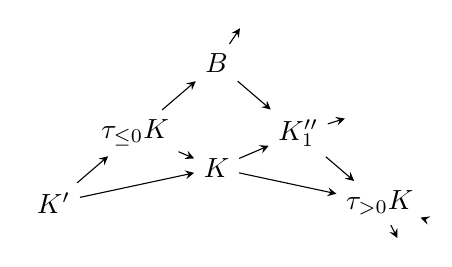
\begin{tikzpicture}[>=stealth,scale=.74]
\node(a)at(0,0){$K'$};\node(b)at(1.4,1.2){$\tau_{\leq0}K$};\node(c)at(2.8,2.4){$B$};\node(d)at(2.8,.6){$K$};\node(e)at(4.2,1.2){$K''_1$};\node(f)at(5.6,0){$\tau_{>0}K$};
\draw[->](a)--(b);\draw[->](b)--(c);\draw[->](c)--(e);\draw[->](e)--(f);\draw[->](a)--(d);\draw[->](b)--(d);\draw[->](d)--(e);\draw[->](d)--(f);\draw[->](c)--++(.4,.6);\draw[->](e)--++(.8,.25);\draw[->](f)--++(.7,-.25);\draw[->](f)--++(.3,-.6);
\end{tikzpicture}
\end{center}
三角 $(B,K''_1,\tau_{>0}K)$ 是 $K''_1$ 的1.3.1(iii)型三角，表明 $K''_1\in\mathcal D^{\geq0}$，且 $H^0K''_1=B$、$\tau_{>0}K\xrightarrow{\sim}\tau_{>0}K''_1$。由(ii)，$K''_1$ 与 $K''$ 等同，因此 $(K',K,K''_1)$ 就是(iii)中所需的三角。

\par\medskip\noindent\textbf{1.3.16.} 设 $\mathcal D_i$（$i=1,2$）是两个 $t$-范畴，$\mathcal C_i$ 是 $\mathcal D_i$ 的\term{heart}{心}，以 $\varepsilon$ 表示包含函子 $\mathcal C_i\hookrightarrow\mathcal D_i$。设 $T:\mathcal D_1\to\mathcal D_2$ 是\term{triangulated-category}{三角范畴}间的\term{exact-functor}{正合函子}（[10] 第4页）。若 $T(\mathcal D_1^{\leq0})\subset\mathcal D_2^{\leq0}$，则称 $T$ 右 \term{t-exact}{$t$-正合}；若 $T(\mathcal D_1^{\geq0})\subset\mathcal D_2^{\geq0}$，则称 $T$ 左 \term{t-exact}{$t$-正合}；同时左、右 \term{t-exact}{$t$-正合}时，称 $T$ 为 \term{t-exact}{$t$-正合}函子。

\par\medskip\noindent\textbf{命题1.3.17。} (i) 若 $T$ 左（相应地，右）\term{t-exact}{$t$-正合}，则加性函子 ${}^pT:=H^0\circ T\circ\varepsilon:\mathcal C_1\to\mathcal C_2$ 左（相应地，右）正合。
\SourcePage{44}
(ii) 若 $T$ 左（相应地，右）\term{t-exact}{$t$-正合}且 $K\in\mathcal D_1^{\geq0}$（相应地，$\mathcal D_1^{\leq0}$），则有 ${}^pTH^0K\xrightarrow{\sim}H^0TK$（相应地，$H^0TK\xrightarrow{\sim}{}^pTH^0K$）。

(iii) 设 $(T^*,T_*)$ 是一对互为\term{adjunction}{伴随}的\term{exact-functor}{正合函子}，其中 $T^*:\mathcal D_2\to\mathcal D_1$，$T_*:\mathcal D_1\to\mathcal D_2$ 是 $T^*$ 的右\term{adjunction}{伴随}。$T^*$ 右 \term{t-exact}{$t$-正合}的充要条件为 $T_*$ 左 \term{t-exact}{$t$-正合}；此时 $({}^pT^*,{}^pT_*)$ 构成一对\term{adjoint-functor}{伴随函子} $\mathcal C_1\rightleftarrows\mathcal C_2$。

(iv) 若 $T_1:\mathcal D_1\to\mathcal D_2$ 与 $T_2:\mathcal D_2\to\mathcal D_3$ 都左（相应地，右）\term{t-exact}{$t$-正合}，则 $T_2\circ T_1$ 也如此，且 ${}^p(T_2\circ T_1)={}^pT_2\circ{}^pT_1$。

若 $T$ 左 \term{t-exact}{$t$-正合}，则对 $\mathcal C_1$ 中每个短\term{exact-sequence}{正合列} $0\to X\to Y\to Z\to0$，\term{distinguished-triangle}{区别三角} $(T(X),T(Y),T(Z))$ 的\term{cohomology}{上同调}长\term{exact-sequence}{正合列}给出 $0\to H^0T(X)\to H^0T(Y)\to H^0T(Z)$，因为 $T(Z)\in\mathcal D_2^{\geq0}$。这就证明了(i)的左正合情形，右正合情形由\term{duality}{对偶}性得到。

对 $K\in\mathcal D_1^{\geq0}$，三角 $(H^0K,K,\tau_{>0}K)$ 给出三角 $(TH^0K,TK,T\tau_{>0}K)$，其中 $T\tau_{>0}K\in\mathcal D_2^{>0}$；其\term{cohomology}{上同调}长\term{exact-sequence}{正合列}给出 $H^0TH^0K\xrightarrow{\sim}H^0TK$。这与其\term{duality}{对偶}命题证明了(ii)。

若 $T_*$ 左 \term{t-exact}{$t$-正合}，对 $U\in\mathcal D_1^{>0}$、$V\in\mathcal D_2^{\leq0}$，有 $\Hom(T^*V,U)=\Hom(V,T_*U)=0$。这对每个 $U$ 都成立，因此 $\tau_{>0}T^*V=0$，即 $T^*V\in\mathcal D_1^{\leq0}$，所以 $T^*$ 右 \term{t-exact}{$t$-正合}。对 $A\in\mathcal C_1$、$B\in\mathcal C_2$，原文接着写为
\[
 H^0T^*B=\tau_{\leq0}T^*B,\qquad H^0T_*A=\tau_{\leq0}T_*A,
\]
从而有函子同构
\[
 \Hom(H^0T^*B,A)\xrightarrow{\sim}\Hom(T^*B,A)
 =\Hom(A,T_*B)\xleftarrow{\sim}\Hom(A,H^0T_*B).
\]
\footnote{译注：这里忠实保留原文的排印。由前述 \term{t-exact}{$t$-正合}性，第一式中的 $\tau_{\leq0}T^*B$ 应为 $\tau_{\geq0}T^*B$；\term{adjunction}{伴随}同构的右侧按对象所属范畴应为 $\Hom(B,T_*A)$ 及 $\Hom(B,H^0T_*A)$。}
这与\term{duality}{对偶}论证一起证明了(iii)。

若 $T_1,T_2$ 都左 \term{t-exact}{$t$-正合}且 $A\in\mathcal C_1$，则 $T_1A\in\mathcal D_2^{\geq0}$；由(ii)，有 ${}^p(T_2\circ T_1)A=H^0T_2T_1A=H^0T_2H^0T_1A$。这与\term{duality}{对偶}论证一起证明了(iv)。

\par\medskip\noindent\textbf{注1.3.18。} (i) 令 $\mathcal D_1^+=\bigcup_n\mathcal D_1^{\geq n}$、$\mathcal D_2^-=\bigcup_n\mathcal D_2^{\leq n}$。结论(iii)对 $T^*:\mathcal D_2^-\to\mathcal D_1$ 和 $T_*:\mathcal D_1^+\to\mathcal D_2$ 仍然成立；这里的“\term{adjunction}{伴随}”指对 $V\in\mathcal D_2^-$、$U\in\mathcal D_1^+$，函子性地有 $\Hom(T^*V,U)=\Hom(V,T_*U)$。证明相同。

(ii) 对 $A\in\mathcal C_1$、$B\in\mathcal C_2$，$(T^*,T_*)$ 与 $({}^pT^*,{}^pT_*)$ 的\term{adjunction}{伴随}箭头满足如下交换图：
\SourcePage{45}
\[
\begin{tikzcd}[ampersand replacement=\&,column sep=large]
 T^*{}^pT_*A\arrow[r]\arrow[d]\&{}^pT^*{}^pT_*A\arrow[d]\\
 T^*T_*A\arrow[r]\&A
\end{tikzcd}
\qquad\text{和}\qquad
\begin{tikzcd}[ampersand replacement=\&,column sep=large]
 B\arrow[r]\arrow[d]\&T_*T^*B\arrow[d]\\
 {}^pT_*{}^pT^*B\arrow[r]\&T_*{}^pT^*B.
\end{tikzcd}
\]

\par\medskip\noindent\textbf{1.3.19.} 设 $T:\mathcal D'\to\mathcal D$ 是\term{triangulated-category}{三角范畴}间的\term{fully-faithful}{全忠实}\term{exact-functor}{正合函子}。$\mathcal D'$ 的一个三角 $\mathrm{tr}$ 若在 $T$ 下的像 $T\mathrm{tr}$ 是\term{distinguished-triangle}{区别三角}，则它自身就是\term{distinguished-triangle}{区别三角}。事实上，取与 $\mathrm{tr}$ 底边相同的\term{distinguished-triangle}{区别三角} $\mathrm{tr}_1$；$T\mathrm{tr}$ 与 $T\mathrm{tr}_1$ 都是底边相同的\term{distinguished-triangle}{区别三角}，故二者同构，因而 $\mathrm{tr}$ 与 $\mathrm{tr}_1$ 同构。

假设 $\mathcal D,\mathcal D'$ 都配备 \term{t-structure}{$t$-结构}且 $T$ 为 \term{t-exact}{$t$-正合}函子。对 $X\in\mathcal D'$，若 $TX\in\mathcal D^{\leq0}$（相应地，$\mathcal D^{\geq0}$），则 $X\in\mathcal D'^{\leq0}$（相应地，$\mathcal D'^{\geq0}$）：这是因为 $X\in\mathcal D'^{\leq0}\Longleftrightarrow\tau_{>0}X=0$，而 $T$ 与 $\tau_{>0}$ 交换；另一情形\term{duality}{对偶}。

反之，若 $\mathcal D'$ 是\term{triangulated-category}{三角范畴} $\mathcal D$ 的全三角子范畴，且 $(\mathcal D^{\leq0},\mathcal D^{\geq0})$ 是 $\mathcal D$ 上的 \term{t-structure}{$t$-结构}，则
\[
 (\mathcal D'^{\leq0},\mathcal D'^{\geq0}):=(\mathcal D'\cap\mathcal D^{\leq0},\mathcal D'\cap\mathcal D^{\geq0})
\]
为 $\mathcal D'$ 上的 \term{t-structure}{$t$-结构}，当且仅当 $\mathcal D'$ 在函子 $\tau_{\leq0}$ 下稳定。满足此条件时，称所得结构为诱导 \term{t-structure}{$t$-结构}。对配备诱导 \term{t-structure}{$t$-结构}的 $\mathcal D'$，包含函子 $\mathcal D'\hookrightarrow\mathcal D$ 为 \term{t-exact}{$t$-正合}函子；有 $\mathcal C'=\mathcal D'\cap\mathcal C$，而 $\mathcal D$ 的函子 $\tau_{\leq p}$、$\tau_{\geq p}$、$H^p$ 限制到 $\mathcal D'$ 后，分别与 $\mathcal D'$ 的同名函子等同。

\par\medskip\noindent\textbf{1.3.20.} 设 $(\mathcal D_i)_{i\in I}$ 是有限族\term{triangulated-category}{三角范畴}，$T:\prod_i\mathcal D_i\to\mathcal D$ 是到\term{triangulated-category}{三角范畴} $\mathcal D$ 的正合多函子（SGA 4 XVII 1.1.3）。假设各 $\mathcal D_i$ 与 $\mathcal D$ 均配备 \term{t-structure}{$t$-结构}。若 $T$ 将各 $\mathcal D_i^{\geq0}$（相应地，$\mathcal D_i^{\leq0}$）的乘积映到 $\mathcal D^{\geq0}$（相应地，$\mathcal D^{\leq0}$），则称它左（相应地，右）\term{t-exact}{$t$-正合}；若左右均成立，则称它 \term{t-exact}{$t$-正合}。若 $T$ 左 \term{t-exact}{$t$-正合}（相应地，右 \term{t-exact}{$t$-正合}，或 \term{t-exact}{$t$-正合}），并将某些变量固定为 $\mathcal D_i^{\geq0}$（相应地，$\mathcal D_i^{\leq0}$，或 $\mathcal D_i$ 的\term{heart}{心} $\mathcal C_i$）中的给定对象，则所得关于其余变量的函子仍具有同样的 \term{t-exact}{$t$-正合}性。这使我们可以将单变量函子的结果应用于 $T$。例如：

令 $\varepsilon_i:\mathcal C_i\hookrightarrow\mathcal D_i$ 为包含函子，置 ${}^pT=H^0\circ T\circ(\varepsilon_i)_{i\in I}$。若 $T$ 左（相应地，右）\term{t-exact}{$t$-正合}，则从各 $\mathcal C_i$ 到 $\mathcal C$ 的加性多函子 ${}^pT$ 左（相应地，右）正合。

假设 $T$ 左 \term{t-exact}{$t$-正合}。对 $K_i\in\mathcal D_i^{\geq0}$，
\SourcePage{46}
由1.3.17(ii)有 ${}^pT(H^0K_i)\xrightarrow{\sim}H^0T(K_i)$。对任意 $K_i$，态射 $K_i\to\tau_{\geq0}K_i$ 给出态射
\begin{equation*}
 H^0T(K_i)\longrightarrow H^0T(\tau_{\geq0}K_i)\xleftarrow{\sim}{}^pT(H^0K_i).\tag{1.3.20.1}
\end{equation*}
作平移后，更一般地，当 $\sum_i n_i=n$ 时，得到态射
\begin{equation*}
 H^nT(K_i)\longrightarrow{}^pT(H^{n_i}K_i).\tag{1.3.20.2}
\end{equation*}
这里有符号问题；若改为考虑
\begin{equation*}
 H^nT(K_i)\longrightarrow H^nT\bigl((H^{n_i}K_i)[-n_i]\bigr),\tag{1.3.20.3}
\end{equation*}
就不会出现这一问题。

若 $T$ 右 \term{t-exact}{$t$-正合}，则对 $K_i\in\mathcal D_i^{\leq0}$ 有 ${}^pTH^0K_i\xleftarrow{\sim}H^0TK_i$；态射 $\tau_{\leq0}K_i\to K_i$ 给出态射 ${}^pT(H^0K_i)\to H^0T(K_i)$，再作平移得到
\begin{equation*}
 H^nT\bigl((H^{n_i}K_i)[-n_i]\bigr)\longrightarrow H^nT(K_i)
 \qquad\left(\sum_i n_i=n\right).\tag{1.3.20.4}
\end{equation*}
若 $T$ 为 \term{t-exact}{$t$-正合}函子，则(1.3.20.3)、(1.3.20.4)同时存在。将 $H^nT$ 应用于交换图
\[
\begin{tikzcd}[ampersand replacement=\&,column sep=large]
 \tau_{\leq n_i}K_i\arrow[r]\arrow[d]\&H^{n_i}K_i[-n_i]\arrow[d]\\
 K_i\arrow[r]\&\tau_{\geq n_i}K_i
\end{tikzcd}
\]
可知复合 $(1.3.20.3)\circ(1.3.20.4)$ 是恒等态射。若 $\sum_i n_i=\sum_i m_i=n$ 且 $(n_i)_{i\in I}\neq(m_i)_{i\in I}$，则存在某个 $i$ 使 $n_i<m_i$。复合 $\tau_{\leq n_i}K_i\to K_i\to\tau_{\geq m_i}K_i$ 为零，因此“$(m_i)$ 对应的(1.3.20.3)”与“$(n_i)$ 对应的(1.3.20.4)”的复合也为零。

\par\medskip\noindent\textbf{命题1.3.21。} 若 $T$ 为 \term{t-exact}{$t$-正合}函子且 $K_i\in\mathcal D_i^b$，则态射(1.3.20.3)和(1.3.20.4)定义互为逆的同构
\begin{equation*}
 H^nT(K_i)\simeq\bigoplus_{\sum_i n_i=n}H^nT\bigl((H^{n_i}K_i)[-n_i]\bigr).\tag{1.3.21.1}
\end{equation*}
我们已经看到，这些态射使右侧成为左侧的一个直和因子。(1.3.21.1)两侧关于每个 $K_i$ 都是\term{cohomological-functor}{上同调函子}（对右侧，这是因为 ${}^pT$ 正合）；(1.3.20.3)与(1.3.20.4)是\term{cohomological-functor}{上同调函子}之间的态射。通过逐次分解，归结为各 $K_i\in\mathcal C_i$ 的情形；此时结论显然。

\SourcePage{47}
\par\medskip\noindent\textbf{1.3.22. \term{t-structure}{$t$-结构}的例子。} （本文后续部分不会使用。）

如1.1.4，设 $A$ 为\term{exact-category}{正合范畴}，$E$ 为其短\term{exact-sequence}{正合列}的集合。假设每个态射 $f:A\to B$ 都有核，且 $\Ker(f)\to A$ 可嵌入短\term{exact-sequence}{正合列} $0\to\Ker(f)\to A\to\mathrm{Coim}(f)\to0$。令 $\mathcal D^{\leq0}$（相应地，$\mathcal D^{\geq0}$）为 $\mathcal D:=DA$（1.1.4）的子范畴，由满足当 $i>0$（相应地，$i<0$）时态射 $\mathrm{Coim}(d^{i-1})\to\Ker(d^i)$ 为同构的\term{complex}{复形} $K$ 组成。用嵌入 $h:A\to(A,E)^{\sim}$（1.1.4）来表述，就是 $K$ 在 $D((A,E)^{\sim})$ 中的像 $h_K$ 属于 $D^{\leq0}$（相应地，$D^{\geq0}$）。来证明 $(\mathcal D^{\leq0},\mathcal D^{\geq0})$ 是 $\mathcal D$ 上的 \term{t-structure}{$t$-结构}。

(a) 对 $K,L\in\mathcal D$，有 $\Hom_{\mathcal D}(K,L)=\varinjlim\Hom_{KA}(K',L')$，极限取遍\term{quasi-isomorphism}{拟同构} $K'\to K$ 与 $L\to L'$ 的\term{homotopy}{同伦}类。若 $K\in\mathcal D^{\leq0}$（相应地，$L\in\mathcal D^{\geq1}$），则可以将 $K'$（相应地，$L'$）限制为满足 $i>0$ 时 $K'^i=0$（相应地，$i<0$ 时 $L'^i=0$）的对象，而仍得到\term{cofinal}{余尾}系统；只须使用\term{quasi-isomorphism}{拟同构} $\tau_{\leq0}K'\to K'$（相应地，$L'\to\tau_{\geq1}L'$），其中 $\tau_{\leq0}$、$\tau_{\geq1}$ 如1.3.2(i)所定义。对这样的 $K',L'$，每个\term{complex}{复形}态射 $f:K'\to L'$ 都为零：它由满足 $df^0=0$ 的 $f^0:K'^0\to L'^0$ 决定，而 $d:L'^0\to L'^1$ 是单态射，故 $f^0=0$。这验证了1.3.1(i)。公理1.3.1(ii)显然。

(b) 对 $K\in KA$，有\term{complex}{复形}短\term{exact-sequence}{正合列} $0\to\tau_{\leq0}K\to K\to\tau_{\geq1}K\to0$。它定义 $DA$ 中的\term{distinguished-triangle}{区别三角}：$\tau_{\leq0}K\to K$ 的\term{cone}{锥}\term{quasi-isomorphism}{拟同构}地映到 $\tau_{\geq1}K$。这验证了1.3.1(iii)。

特别地，$\mathcal D$ 的\term{heart}{心} $\mathcal C$ 是\term{abelian-category}{阿贝尔范畴}。$\mathcal C$ 的对象可表示为长为1的\term{complex}{复形} $K^{-1}\xrightarrow{d}K^0$，其中 $d$ 是单态射。对这样的 $K,L$，一个\term{complex}{复形}态射 $f:K\to L$ 由其分量 $f^0:K^0\to L^0$ 唯一确定。若将 $K^{-1}$、$L^{-1}$ 分别与 $K^0$、$L^0$ 的子对象等同，则 $f^0:K^0\to L^0$ 来自\term{complex}{复形}态射 $f$ 当且仅当 $f^0(K^{-1})\subset L^{-1}$；而 $f$ \term{homotopy}{同伦}于零，当且仅当 $f^0(K^0)\subset L^{-1}$。$f$ 是\term{quasi-isomorphism}{拟同构}，意味着列
\[
 0\longrightarrow K^{-1}\longrightarrow K^0\oplus L^{-1}\longrightarrow L^0\longrightarrow0
\]
正合，即 $K^0\oplus L^{-1}\to L^0$ 是\term{admissible}{容许}满态射，且 $K^0$ 的子对象 $K^{-1}$ 是 $L^{-1}$ 沿 $f^0$ 的拉回。

容易验证，若 $K'\xrightarrow{\varphi}K$ 是一个\term{quasi-isomorphism}{拟同构}，
\SourcePage{48}
其中 $K'$ 集中于0次与 $-1$ 次，且 $f\varphi$ \term{homotopy}{同伦}于零（即 $f\varphi(K'^0)\subset L^{-1}$），则 $f$ 也\term{homotopy}{同伦}于零。群 $\Hom_{\mathcal C}(K,L)$ 是如下群关于这种\term{quasi-isomorphism}{拟同构} $\varphi:K'\to K$ 的归纳极限：
\[
 \Hom_{KA}(K',L)=
 \frac{\{f:K'^0\to L^0\mid f(K'^{-1})\subset L^{-1}\}}
 {\{f\mid f(K'^0)\subset L^{-1}\}};
\]
而此归纳极限中的过渡态射都是单射。

\par\medskip\noindent\textbf{1.3.23. 习题。} (i) 对 $A$ 中对象的\term{complex}{复形} $K$，$\mathcal C$ 中的 $H^0K$ 是\term{complex}{复形} $\mathrm{Coim}(d^{-1})\to\Ker(d^0)$。

(ii) 若函子 $F$ 从 $A$ 到\term{abelian-category}{阿贝尔范畴} $N$，并将 $E$ 中的列变为右\term{exact-sequence}{正合列} $FA\to FB\to FC\to0$，则它可唯一地（在唯一同构意义下）延拓为右\term{exact-functor}{正合函子} $F':\mathcal C\to N$。若 $F$ \term{fully-faithful}{全忠实}，并将 $E$ 中的列变为短\term{exact-sequence}{正合列}，将单态射变为单态射，则 $F'$ 正合且\term{fully-faithful}{全忠实}。特别地，复合函子
\[
 \mathcal C\longrightarrow DA\longrightarrow D((A,E)^{\sim})\xrightarrow{H^0}(A,E)^{\sim}
\]
是\term{fully-faithful}{全忠实}的；它将 $\mathcal C$ 与 $(A,E)^{\sim}$ 中由一个 $A$ 的对象除以一个仍属于 $A$ 的子对象所得的商组成的范畴等同。

(iii) 函子 $D^-A\to D^-\mathcal C$ 是\term{equivalence}{等价}（上标 $-$ 表示只考虑有上界的\term{complex}{复形}）。［利用每个 $\mathcal C$ 的对象都是某个 $A$ 的对象的商。］

(iv) 设 $A$ 是\term{abelian-category}{阿贝尔范畴}。$FA$ 满足1.3.22的假设（1.1.3例2）。设 $\mathcal C$ 是相应的\term{filtration}{滤过}对象的\term{formal-quotient}{形式商}所成的\term{abelian-category}{阿贝尔范畴}；设 $\mathcal C'$ 为列 $\cdots\to A^i\to A^{i-1}\to\cdots$ 所成的范畴，其中 $i\gg0$ 时 $A^i=0$，$i\ll0$ 时 $A^i\xrightarrow{\sim}A^{i-1}$。证明从 $\mathcal C$ 到 $\mathcal C'$ 的函子
\[
 ((V^{-1},F)\longrightarrow(V^0,F))\longmapsto
 \bigl(\Coker(F^iV^{-1}\to F^iV^0)\bigr)_i
\]
是\term{equivalence}{等价}。［应用(ii)。］

\par\medskip\noindent\textbf{1.3.24. 例。} 取 $A$ 为 Banach 空间范畴，将忘掉拓扑后变为短\term{exact-sequence}{正合列}的列作为短\term{exact-sequence}{正合列}，则1.3.22的假设成立。由\term{closed-graph-theorem}{闭图像定理}，这些列就是同构于 $0\to A\to B\to C\to0$ 的列，其中 $A$ 是 $B$ 的闭子空间，$C=B/A$。所得范畴 $\mathcal C$ 是“\term{formal-quotient}{形式商}” $B/A$ 所成的范畴（这里 $A\to B$ 是 Banach 空间之间的连续单射线性映射）。\term{closed-graph-theorem}{闭图像定理}保证：若\term{complex}{复形} $K^{-1}\to K^0$ 与 $L^{-1}\to L^0$ 定义 $\mathcal C$ 的对象，则一个\term{complex}{复形}态射 $f:K\to L$ 等同于连续线性映射 $f^0:K^0\to L^0$，且在集合意义下 $f(K^{-1})\subset L^{-1}$；而 $f$ \term{homotopy}{同伦}于零（即在 $\mathcal C$ 中为零），当且仅当在集合意义下 $f(K^0)\subset L^{-1}$。
\SourcePage{49}
L. Walbroeck 曾考虑过类似的\term{formal-quotient}{形式商}（\emph{Les quotients de b-espaces}，预印本，Bruxelles，1962）。
